\documentclass[DIV=14,headsepline,footsepline]{scrbook}
% header_phys_en.tex
% ----------------------------------------------------
% Lädt alle Header-Dateien für physikalische Dokumente
% ====================================================
% SPRACHE: ENGLISCH
% (Reihenfolge nicht ändern -> Führt sonst zu Fehlern)
%
% package_en.tex
% --------------------------------------------
% Headerdatei, die alle nötigen Packages lädt.
% ============================================
% SPRACHE: ENGLISCH
%
%  		Festlegen der Zeichencodierung des Dokuments und des Zeichensatzes.
%     Wir verwenden 'uft8' für das Dokument, da wir seit TxC standardmäßig UTF8-Dokumente erzeugen. Als Legacy-Option kann auch 'Latin1' 
%			(ISO-8859-1) für das Dokument gesetzt werden, wenn die Dateien in ANSI-Codierunge gespeichert werden.
%     Außerdem 'T1' Codierung für die Schrift.
%
\usepackage[utf8]{inputenc}
\usepackage[T1]{fontenc}
%
%  		Paket für die Lokalisierung ins Deutsche laden.
%     Wir verwenden neue deutsche Rechtschreibung mit 'ngerman'.
%
\usepackage[ngerman, english]{babel}
%
% 		Paket für Farben an verschieden Stellen. 
%     Wir definieren zusätzliche benannte Farben im 'style-header'.
%
\usepackage{color}
%
%			Paket für das Layout der Literaturangabe und 'Deutsche' Literaturangaben.
%
\usepackage[sort&compress, numbers]{natbib}
%
%			Paket für die \subfloat[]{}-Umgebung.
%
\usepackage[margin=1em, indention=1em]{subfig}
%
% 		Das Hyperref-Package verwenden. Spezielle Optionen werden gesondert erläutert.
%
\usepackage[
	pdfauthor={cand. phys. Erik Hänel},%				     											Autor des PDF Dokuments.
	pdfcreator={MiKTeX, LaTeX with hyperref and KOMA-Script},% 								Erzeuger/Kompiler des PDF Dokuments.
	bookmarksopenlevel={sections},%															 								PDF-Lesezeichen bis zu Sections öffnen.
	pdfpagemode={UseOutlines},%                                  								PDF-Lesezeichen beim Öffnen anzeigen.
	pdfdisplaydoctitle={true},%                                  								Dokumenttitel statt Dateiname in der Titelzeile anzeigen.
	pdfstartview={FitH}%																			 								Größe an Fensterbreite anpassen
]{hyperref}
%
%			Das Caption-Paket erlaubt, die Bildunterschriften der \subfloat[]{}-Umgebung zu formatieren.
%
\usepackage{caption}
\usepackage{array}		
\usepackage{graphicx}
\usepackage{epsfig}
%
%			AMS-MATH-Package mit der Option, die Grenzen bei Summen, Integralen und anderen Operatoren immer über und unter dem Symbol anzuzeigen.
%
\usepackage[sumlimits,intlimits,namelimits]{amsmath}
%
%			AMS-Packages für spezielle Symbole und Kommutative Diagramme
%
\usepackage{amssymb,amscd}
%
%			Symbole für Körper und Mengen (C,R,N,Q,etc.)
%
\usepackage{dsfont}
%
%			Schriftartensetup: Palatino für Textsatz und Pazomath für Mathesatz
%
\usepackage{mathpazo}
%
%			Schriftartensetup: Helvetica als serifenlose Schriftart und Courier für \texttt{}
%
\usepackage[scaled = 0.95]{helvet}
\usepackage{courier}
%
%			Spezialpackage: Erlaubt es, sich eigene Mathe-Akzente zu definieren. Findet hier bei dem Befehl \vhat{} Anwendung, der ein Hütchen mit 
%			einem Pfeil kombiniert.
%
\usepackage{accents}
%
%			Erweitert die Darstellung von Tabellen mit den Befehlen \toprule, \midrule & \bottomrule
%
\usepackage{booktabs}
%
%			Dieses Package wird für den Befehl \mum verwendet, der 'µm' als Einheit definiert.
%
\usepackage{textcomp}
%
% ========================================================
% EOF
%
% style_phys.tex
% -------------------------------------------------------------------
% Headerdatei, die das Aussehen und das Layout der Dokumente steuert.
% ===================================================================

%
%  1. Definieren von eigenen benannten Farben.
%     Für spätere Verwendung in dem Dokument, definieren wir einzelne
%     benannte Farben. Sie finden bei den Links, den Überschriften und die spezielle
%			'shadecolor' bei den farbigen Boxen (mit '\begin{shaded}\end{shaded}' gesetzt) Verwendung.
%
\definecolor{LinkColor}{rgb}{0,0,0.6}
\definecolor{HeadColor}{rgb}{0,0,0.5}
\definecolor{shadecolor}{rgb}{0.85,0.95,1}

%
%  2. KOMA-Script Option, Zeilenumbruch bei Bildbeschreibungen.
%
\setcapindent{1em}

%
%  3. Stil der Kopf- und Fusszeilen.
%     Wir aktivieren mit 'headings' laufende Seiten- /Kolumnentitel.
%
\pagestyle{headings}

%
%  4. Definieren der Schriftarten/Schiftfamilien der einzelnen Bereiche.
%
\setkomafont{chapter}{\huge\scshape\color{HeadColor}}       				% Kapitel farbig, Groß und als Kapitälchen
\setkomafont{section}{\Large\color{HeadColor}}											% Sections farbig und größer als normal
\setkomafont{captionlabel}{\sffamily\bfseries\color{HeadColor}}     % Fette Beschriftungstitel, farbig und serifenlos 
\setkomafont{caption}{\sffamily}																		% serifenlose Beschriftungen (tables/figures)
\setkomafont{pagehead}{\sffamily\bfseries\color{HeadColor}}         % Kolumnentitel serifenlos, farbig und fett
\setkomafont{descriptionlabel}{\sffamily\bfseries} 									% Fette und serifenlose Beschreibungstitel
\setkomafont{pagenumber}{\sffamily\bfseries}												% Fette, serifenlose Seitenzahlen
\setkomafont{part}{\Huge\scshape\color{HeadColor}}									% 'Part'-Titel Riesig, Kapitälchen und farbig

% Layouteinstellungen für "Subfloats": \subfloat[Titel]{\includegraphics[width=0.5\textwidth]{Pfad/zur/bilddatei.endung}}
\captionsetup[subfigure]{font={sf,footnotesize}, labelformat=simple, labelsep=colon}

%
%  5. Farbeinstellungen für die Links im PDF Dokument.
%
\hypersetup{%
	colorlinks=true,%        Aktivieren von farbigen Links im Dokument (keine Rahmen)
	linkcolor=LinkColor,%    Farbe festlegen.
	citecolor=LinkColor,%    Farbe festlegen.
	filecolor=linkColor,%    Farbe festlegen.
	menucolor=LinkColor,%    Farbe festlegen.
	urlcolor=LinkColor,%     Farbe von URL's im Dokument.
	bookmarksnumbered=true%  Überschriftsnummerierung im PDF Inhalt anzeigen.
}

%%%%%%%%%%%%%%%%%%%%%%%%%%%%%%%%%%%%%%%%%%%%%%%%%%%%%%%%%%%%
%
%  6. Die Besondere Formatierung der Kapitelüberschriften (Linien drüber und drunter)
%
 
% 1st get a new command
\newcommand*{\ORIGchapterheadstartvskip}{}%
% 2nd save the original definition to the new command
\let\ORIGchapterheadstartvskip=\chapterheadstartvskip
% 3rd redefine the command using the saved original command
\renewcommand*{\chapterheadstartvskip}{%
  \ORIGchapterheadstartvskip
  {%
    \setlength{\parskip}{0pt}%
    \noindent\rule[.3\baselineskip]{\linewidth}{1pt}\par
  }%
}
 
% see above
\newcommand*{\ORIGchapterheadendvskip}{}%
\let\ORIGchapterheadendvskip=\chapterheadendvskip
\renewcommand*{\chapterheadendvskip}{%
  {%
    \setlength{\parskip}{0pt}%
    \noindent\rule[.3\baselineskip]{\linewidth}{1pt}\par
  }%
  \ORIGchapterheadendvskip
}
%
%  End of chapter head change
%
%%%%%%%%%%%%%%%%%%%%%%%%%%%%%%%%%%%%%%%%%%%%%%%%%%%%%%%%%%%%
%
% ===========================================================================
% EOF
%
%	command.tex
% -------------------------------------------
%	Headerdatei, die alle nötigen Befehle lädt.
% ===========================================
%
% QM-spezifische Befehle: \bra{} (\tbra{}), \ket{} (\tket{}), \skal{}{} (\tskal{}{}) [Skalarprodukt], \EW{}, \ew{} [Erwartungswert]
%
\newcommand{\bra}[1]{\left\langle #1 \right|}
\newcommand{\tbra}[1]{\langle #1|}
\newcommand{\ket}[1]{\left| #1\right\rangle}					
\newcommand{\tket}[1]{| #1 \rangle}										
\newcommand{\skal}[2]{\left\langle #1 | #2 \right\rangle}
\newcommand{\tskal}[2]{\langle #1|#2\rangle}					
\newcommand{\EW}[1]{\left\langle #1 \right\rangle}		
\newcommand{\ew}[1]{\langle #1\rangle}
\newcommand{\vhat}[1]{\accentset{\hspace{1.6pt}\text{\fontsize{4.5pt}{4pt}{$\boldsymbol\wedge$}}\hspace{-3.9pt}\text{\fontsize{5pt}{4pt}{$\boldsymbol{\rightarrow}$}}}{#1}\hspace{0.4pt}}
%
% Allg. mathematische Befehle: \msakl [Skalarprodukt: <*,*>], \dx, \e, \eps, \prt{}{}, \Diff{}, \diff{}{}, \svec{}, \abs{}, \norm{}, \rot, 
%	\laplace
%
\newcommand{\mskal}[2]{\left\langle #1 , #2 \right\rangle}
\newcommand{\dx}{\:\mathrm{\normalfont{d}}}
\newcommand{\e}[1]{\:\mathrm{\normalfont{e}}^{#1}}
\newcommand{\eps}{\varepsilon}
\newcommand{\prt}[2]{\frac{\partial #1}{\partial #2}}
\newcommand{\diff}[2]{\frac{\mathrm{d} #1}{\mathrm{d} #2}} 
\newcommand{\Diff}[1]{\diff{}{#1}}									
\newcommand{\svec}[1]{\begin{pmatrix} #1 \end{pmatrix}} 
\newcommand{\detm}[1]{\begin{vmatrix} #1 \end{vmatrix}}
\newcommand{\abs}[1]{\left|#1\right|}									
\newcommand{\norm}[1]{\left\|#1\right\|}
\DeclareMathOperator{\rot}{rot}
\DeclareMathOperator{\divergence}{div}
\DeclareMathOperator{\erfc}{erfc}
\DeclareMathOperator{\erf}{erf}
\newcommand{\laplace}{{}\hspace{-0.3em}\mathrel{\rotatebox[origin=c]{180}{$\nabla$}}\hspace{-0.3em}}
%
% Abkürzungen für Mathematische Körper und Mengen
%
\newcommand{\N}{\mathds N}
\newcommand{\Z}{\mathds Z}
\newcommand{\R}{\mathds R}
\newcommand{\Q}{\mathds Q}
\newcommand{\C}{\mathds C}
\newcommand{\K}{\mathds K}
\newcommand{\V}{\mathds V}
\newcommand{\I}{\Im}
%
% Definition für µm
%
\newcommand{\mum}{\textmu m}
%
% Für Isotopenschreibweise von Elementen/Nukliden z.B. \chem{12}{6}C (Im gewöhnlichen Text)
% 
\newcommand{\chem}[2]{\shortstack[r]{\tiny{${#1}$}\\\scriptsize{$_{#2}$}}}
\newcommand{\sufo}[1]{\ensuremath{\mathrm{#1}}}
%
% Aufrecht gesetzter Indextext
%
\newcommand{\tx}[1]{_{\mathrm{#1}}}
%
% Der \vldt{} Befehl: Zeichet eine Linie, die das Argument als eine Marginalie auf dem Rand und über dem Strich darstellt. Spezialbefehl zum 
%	Datums-Ordnen von Vorlesungskripten
%
\newcommand{\vldt}[1]{\rule{0mm}{8mm}\textsf{\small{\textcolor{HeadColor}{$\blacktriangledown$ \textbf{Vorlesung vom #1}}}}
\marginline{\fbox{\textsf{\textbf{\small{\textcolor{HeadColor}{#1}}}}}}\newline\rule[.75\baselineskip]{\linewidth}{0.5pt}}
%
% Der \helpidx{} Befehl: Zeichet eine Linie, die das Argument als eine Marginalie auf dem Rand und über dem Strich darstellt. Spezialbefehl zum 
%	Datums-Ordnen von Vorlesungskripten
%
\newcommand{\helpidx}[1]{\noindent\rule{0mm}{5mm}\textsf{{\footnotesize\textcolor{HeadColor}{$\blacktriangleright$ \textbf{In the \textsc{NumeRe} documentation at:}}}} {\footnotesize\texttt{help #1}}
\marginline{\fbox{\texttt{\scriptsize{\textcolor{HeadColor}{#1}}}}}\newline\rule[.75\baselineskip]{\linewidth}{0.5pt}}
%
% Der \cmd{} Befehl: Zeichet eine Linie, die das Argument als eine Marginalie auf dem Rand und über dem Strich darstellt. Spezialbefehl zum 
%	Datums-Ordnen von Vorlesungskripten
%
\newcommand{\cmd}[1]{\marginline{\scriptsize\textsf{Syntax element}\\\texttt{\textbf{\scriptsize{\textcolor{red}{#1}}}}}}
%
%  Abkürzung für den \displaybreak[1]. Mit diesem Befehl kann man 'align'-Umgebungen beim Seitenende gezielt umbrechen.
%
\newcommand{\br}{\displaybreak[1]}
%
% Eine Erweiterung des \ref{label}-Befehls: Generiert einen Link, der Aus Objekttyp, Objektidentifikator und Objektcaption zusammengesetzt ist. 
% Bietet sich für Bezüge auf Abschnitte an: \fullref{sec:abschnitt} produziert z.B. 'Abschnitt 1.1 Abschnittstitel'
%
\newcommand{\fullref}[1]{\autoref{#1}: \nameref{#1}}
%
% Umgebung für eine alphabetisch nummerierte Liste
%
\newcounter{ale}
\newcommand{\abc}{\item[\alph{ale})]\stepcounter{ale}}
\newenvironment{liste}{\begin{itemize}}{\end{itemize}}
\newcommand{\aliste}{\begin{liste} \setcounter{ale}{1}}
\newcommand{\zliste}{\end{liste}}
\newenvironment{abcliste}{\aliste}{\zliste}
%	Setzen mit '\aliste\abc Text \zliste'
%
% ============================================
% EOF
%


% ====================================================
% EOF
%
\usepackage{xcolor}
\usepackage{inconsolata}

\hypersetup{
	pdftitle={NumeRe Documentation},
	pdfsubject={NumeRe Documentation}
	}

\usepackage{listings}


\lstdefinelanguage{nscr}
{
	keywordsprefix=$,
	alsoletter={~\#},
	keywords=[1]{},
	keywords=[2]{abort,about,append,audio,break,clear,compose,cont,cont3d,continue,contour,contour3d,copy,credits,datagrid,define,del,delete,dens,dens3d,density,density3d,diff,draw,draw3d,edit,eval,explicit,export,extrema,fft,find,fit,fitw,get,global,grad,gradient,grad3d,gradient3d,graph,graph3d,help,hist,hist2d,hline,ifndef,ifndefined,info,install,integrate,integrate2,integrate2d,list,load,man,matop,mesh,mesh3d,meshgrid,meshgrid3d,move,mtrxop,new,odesolve,plot,plot3d,print,progress,pulse,quit,random,read,redef,redefine,regularize,reload,remove,rename,repl,replaceline,resample,retoque,save,script,search,set,show,showf,smooth,sort,stats,start,stfa,subplot,surf,surf3d,surface,surface3d,swap,taylor,undef,undefine,uninstall,vect,vect3d,vector,vector3d,view,workpath,write,zeroes,else,elseif,endfor,endif,endwhile,endcompose,explicit,for,if,readline,while,spline,namespace,return,throw,str,var,tab,procedure,endprocedure,private,inline},
	keywords=[3]{abs,acos,acosh,Ai,and,arc,arcv,arccos,arcsin,arctan,arcosh,arsinh,artanh,asin,asinh,ascii,atan,atanh,avg,bessel,betheweizsaecker,Bi,binom,char,circle,clock,cmp,cnt,cone,conev,cos,cosh,cot,cross,cuboid,curve,date,dblfacul,degree,det,diag,diagonalize,drop,eigenvals,eigenvects,ellipse,ellipsev,ellipticD,ellipticE,ellipticF,ellipticPi,erf,erfc,exp,face,facev,faculty,findfile,findparam,floor,gamma,gauss,gcd,getfilelist,getfolderlist,getindices,getmatchingparens,getopt,heaviside,hermite,identity,imY,invert,ivl,is_data,is_nan,is_string,laguerre,laguerre_a,lcm,legendre,legendre_a,ln,log,log10,log2,matfc,matfcf,matfl,matflf,max,med,min,neumann,norm,num,one,or,pct,phi,point,polygon,polygonv,prd,radian,rand,range,rect,repeat,replace,replaceall,reshape,resize,rint,roof,round,sbessel,sign,sin,sinc,sinh,size,sneumann,solve,split,sphere,sqrt,std,strfnd,string_cast,strlen,strmatch,str_not_match,str_not_rmatch,strrfnd,strrmatch,student_t,substr,sum,tan,tanh,text,theta,time,to_char,to_cmd,to_lowercase,to_string,to_uppercase,to_value,trace,tracev,transpose,triangle,trianglev,valtostr,version,Y,Z,zero},
	keywords=[4]{_pi,_2pi,_g,_R,_alpha_fs,_c,_coul_norm,_elek_feldkonst,_elem_ladung,_G,_h,_hbar,_k_boltz,_m_amu,_m_elektron,_m_erde,_m_muon,_m_neutron,_m_proton,_m_sonne,_m_tau,_magn_feldkonst,_mu_bohr,_mu_kern,_n_avogadro,_r_bohr,_r_erde,_r_sonne,_theta_weinberg,_mu_e,_mu_p,_mu_n,_stefan_boltzmann,_wien,_rydberg,_hartree,_lande_e,_gamma_e,_gamma_p,_gamma_n,_feigenbaum_delta,_feigenbaum_alpha},
	keywords=[5]{addxaxis,addyaxis,adventor,all,allmedium,alpha,alphamask,animate,app,area,aspect,asstr,asval,autosave,avg,axis,axisbind,background,bar,bars,bcancel,bgcolorscheme,binlabel,binomial,bins,bonum,bottomleft,bottomright,box,boxplot,buffersize,cancel,cartesian,chimap,chorus,clog,cloudplot,cmd,cnt,coarse,coast,cold,colorbar,colormask,colorrange,colorscheme,colortheme,cols,comment,comments,compact,complete,complex,connect,const,copper,coords,countlabel,crust,cscale,cticklabels,cticks,cursor,cut,defcontrol,desc,dir,distrib,down,draftmode,editor,eps,errorbars,every,exprvar,extendedfileinfo,externaldocwindow,faststart,fcont,file,files,fine,first,flength,flow,font,free,freedman,freedoms,func,fx0,gamma,gauss,greeting,grey,grid,gridstyle,hbars,head,heros,heroscn,hints,hires,hot,html,ignore,interpolate,inverse,iter,keepdim,last,lborder,lcont,legend,legendstyle,light,lines,linesizes,linestyles,lnumctrl,loademptycols,loadpath,logic,logscale,lyapunov,main,map,marks,mask,max,maxline,mean,med,medium,method,min,minline,mode,moy,msg,multiplot,noalpha,noalphamask,noanimate,noarea,noaxis,nobackground,nobars,nobox,noboxplot,noclog,nocloudplot,nocolorbar,nocolormask,noconnect,nocrust,nocut,noerrorbars,nofcont,noflength,noflow,nogrid,nohbars,nohires,nointerpolate,nolcont,nolight,nologscale,nomarks,noopen,noorthoproject,nopcont,nopipe,nopoints,noquotes,norefresh,noregion,norm,normal,noschematic,nosteps,nosilent,noxerrorbars,noxlog,noyerrorbars,noylog,nozlog,nq,num,oeps,ogif,onlycolors,onlystyles,open,opng,order,origin,orthoproject,osvg,otex,override,overwrite,pagella,params,pattern,pcont,peek,perspective,pipe,plasma,plotcolors,plotfont,plotparams,plotpath,plugin,plugins,points,pointstyles,poisson,polar,polar_pz,polar_rp,polar_rz,prd,precision,prob,proc,procpath,rainbow,rborder,real,recursive,refresh,region,reset,restrict,rk2,rk4,rk8pd,rkck,rkf45,rotate,samples,savepath,saverr,scale,schematic,schola,scott,scriptpath,settings,shape,silent,simpson,single,slices,sliding,spherical,spherical_pt,spherical_rp,spherical_rt,std,steps,student,styles,sum,sv,target,termes,textsize,this,thisfile,title,tocache,tol,topleft,topright,transpose,trapezoidal,trunc,type,ubound,uniform,unique,units,up,usecustomlang,useescinscripts,var,viridis,viewer,vline,width,windowsize,with,xerrorbars,xlabel,xlog,xscale,xticklabels,xticks,xvals,xy,xz,yerrorbars,ylabel,ylog,yscale,yticklabels,yticks,zlabel,zlog,zscale,zticklabels,zticks},
	sensitive=true,
	morecomment=[s]{\#*}{*\#},
	morecomment=[l][commentstyle]{\#\#},
	string=[b]"
}
\newcommand\realnumberstyle[1]{\tiny}
\makeatletter
\newcommand{\zebra}[3]{%
    {\realnumberstyle{#3}}%
    \begingroup
    \lst@basicstyle
    \ifodd\value{lstnumber}%
        \color{#1}%
    \else
        \color{#2}%
    \fi
        \rlap{\hspace*{\lst@numbersep}%
        \color@block{\linewidth}{\ht\strutbox}{\dp\strutbox}%
        }%
    \endgroup
}
\makeatother

\definecolor{ProcedureStyle}{RGB}{128,0,0}
\definecolor{CommandStyle}{RGB}{0,128,255}
\definecolor{StringStyle}{RGB}{128,128,255}
\definecolor{BGColorTwo}{RGB}{245,245,245}
\definecolor{BGColorOne}{RGB}{230,230,230}
\definecolor{CommentStyle}{RGB}{0,128,0}
\definecolor{ConstantStyle}{RGB}{255,0,128}
\definecolor{OptionStyle}{RGB}{0,128,100}
\lstset{
	language=nscr,
	basicstyle={\small\ttfamily},
	extendedchars=true,
	tabsize=4,
	columns=fixed,
	keepspaces=false,
	breaklines=true,
	showstringspaces=false,
	numbers=left, numberstyle=\tiny, stepnumber=2, numbersep=5pt,
	commentstyle={\color{CommentStyle}\bfseries},
	keywordstyle=[1]{\color{ProcedureStyle}\bfseries},
	keywordstyle=[2]{\color{CommandStyle}\bfseries\underbar},
	keywordstyle=[3]{\color{blue}\bfseries},
	keywordstyle=[4]{\color{ConstantStyle}\bfseries},
	keywordstyle=[5]{\color{OptionStyle}},
	stringstyle=\color{StringStyle},
	backgroundcolor=\color{BGColorTwo},
}





\newcommand{\NR}{\textsc{Nu\-me\-Re}}

\begin{document}
	\subject{Documentation}
	\title{\textsc{\textcolor{HeadColor}{NumeRe: Framework für Numerische Rechnungen}}}
	\subtitle{1.1.x-Series\\Free numerical software released under the GNU GPL v3}
	\author{Erik Hänel et al.}
	\publishers{
\includegraphics[width=0.5\textwidth]{_graphics/folder.png}}
	\dedication{\emph{For the friends of science}}
	\maketitle
	\tableofcontents
	
	\addchap{Legal Information}
		\addsec{GNU Free Documentation Licence v1.2}
			{\scriptsize--- Licence of this document ---}\smallskip\\
			\textbf{Copyright \copyright\ 2017, Erik Hänel.}
			
			Permission is granted to copy, distribute and/or modify this document under the terms of the GNU Free Documentation License, Version 1.2 or any later version published by the Free Software Foundation; with no Invariant Sections, no Front-Cover Texts, and no Back-Cover Texts. A copy of the license may be found at \href{http://www.gnu.org/copyleft/fdl.html}{GNU Free Documentation Licence}.
		\addsec{GNU General Public Licence v3}
			{\scriptsize--- Licence of the application and the displayed code fragments ---}\smallskip\\
			\textbf{Copyright \copyright\ 2017, Erik Hänel et al.}
			
			The described application and the listed code fragments are free software: you can redistribute it and/or modify it under the terms of the GNU General Public License as published by the Free Software Foundation, either version 3 of the License, or (at your option) any later version.

			This program is distributed in the hope that it will be useful, but WITHOUT ANY WARRANTY; without even the implied warranty of MERCHANTABILITY or FITNESS FOR A PARTICULAR PURPOSE. See the GNU General Public License for more details.

			You should have received a copy of the GNU General Public License along with this program. If not, see \href{http://www.gnu.org/licenses/}{www.gnu.org/licenses/}.
		\addsec{Team}
			\begin{itemize}
				\item \textbf{Project lead:} Erik \textsc{Hänel}
				\item \textbf{Concept/UI:} Erik \textsc{Hänel}, Chameleon Team
				\item \textbf{Mathematical parser:} Ingo \textsc{Berg}, Erik \textsc{Hänel} (muParser)
				\item \textbf{Plotting:} Alexey \textsc{Balakin} (MathGL)
				\item \textbf{Numerical algorithms:} GNU Scientific Library, Erik \textsc{Hänel}, Alexey \textsc{Balakin}
				\item \textbf{Tokenizer:} Boost-Library
				\item \textbf{Matrix algorithms:} Eigen-Library
				\item \textbf{XML parser:} Lee \textsc{Thomason} (TinyXML-2)
				\item \textbf{Excel-(97-2003)-Functionality:} \textsc{Yap Chun} Wei (BasicExcel)
				\item \textbf{Testing:} C.~\textsc{Alonso}, D.~\textsc{Bammert}, J.~\textsc{Hänel}, R.~\textsc{Hutt}, K.~\textsc{Kilgus}, E.~\textsc{Kloster}, K.~\textsc{Kurz}, M.~\textsc{Löchner}, L.~\textsc{Sahinov\'c}, D.~\textsc{Schmid}, V.~\textsc{Sehra}, G.~\textsc{Stadelmann}, R.~\textsc{Wanner}, A.~\textsc{Winkler}, F.~\textsc{Wunder}, J.~\textsc{Zinßer}
			\end{itemize}
	\addchap{Installation}
		Since the version v1.0.7 >>Bose<< \NR\ is released as an installer on \href{https://sourceforge.net/projects/numere/files/latest/download}{SourceForge}. To install \NR\ on your own computer, just download the installer and execute it. After following the corresponding steps, \NR\ will be installed on your machine and may be executed afterwards.
		
		To install a newer version of \NR\ just install the newer version of \NR\ ontop of the previous one. Do \emph{not} uninstall the previous version, otherwise all your settings will get lost.
		\paragraph{Note}
			The installer nominates >>C:/Software/NumeRe<< as default installing path. This path may be changed to your needs, however you should avoid using the standard >>C:/Program Files/\ldots<< or >>C:/Program Files (x86)/\ldots<<, respectively. \NR\ probably cannot be executed correctly at these locations.
		\addsec{System Preconditions}
			\NR\ may be executed on all desktop version of MS-Windows from Windows XP to Windows 10. For Windows 8.1 and 10 the additional component compatibility has to be installed. Otherwise there are possible crashes during the plotting process.
			
			\NR\ also requires a keyboard for correct execution. The on-screen keyboard may be used as well, though resulting in quite uncomfortable interaction.
		\addsec{Portable and Stable Version}
			As default the installation of the stable version is recommended, which will create the file links for \NR. This requires admin permissions. The portable version may be executed without any admin permissions, however it won't create any file links. \NR-Portable may be started out of any directory, moved to an arbitrary location and simply can be deleted if it shall be uninstalled.
			\paragraph{Note}
				The >>Stable Version<< installer only writes the file links and the link to the uninstaller into the windows registry. No configuration values or other relevant data for execution are written to the registry.
	\part{Basic Usage}
		\chapter{First Steps}
			Most beginnings are not really easy. This is quite obvious, therefore we gathered all relevant first things, which shall make the beginning of the Work with \NR\ as easy as possible. But this documentation doesn't claim that it might by complete. All these possible options and their values are not described here. Their description may be found in the integrated documentation.
			\paragraph{Note}
				This documentation is supported with marginal texts, which shall point to actions inside \NR. Marginal texts printed in read are syntax elements, which may be entered into the \NR\ console. Bordered and dark blue marginal texts name articles in the integrated \NR\ documentation.
			\section{The User Interface}
				\begin{figure}[htb]%
					\centering
					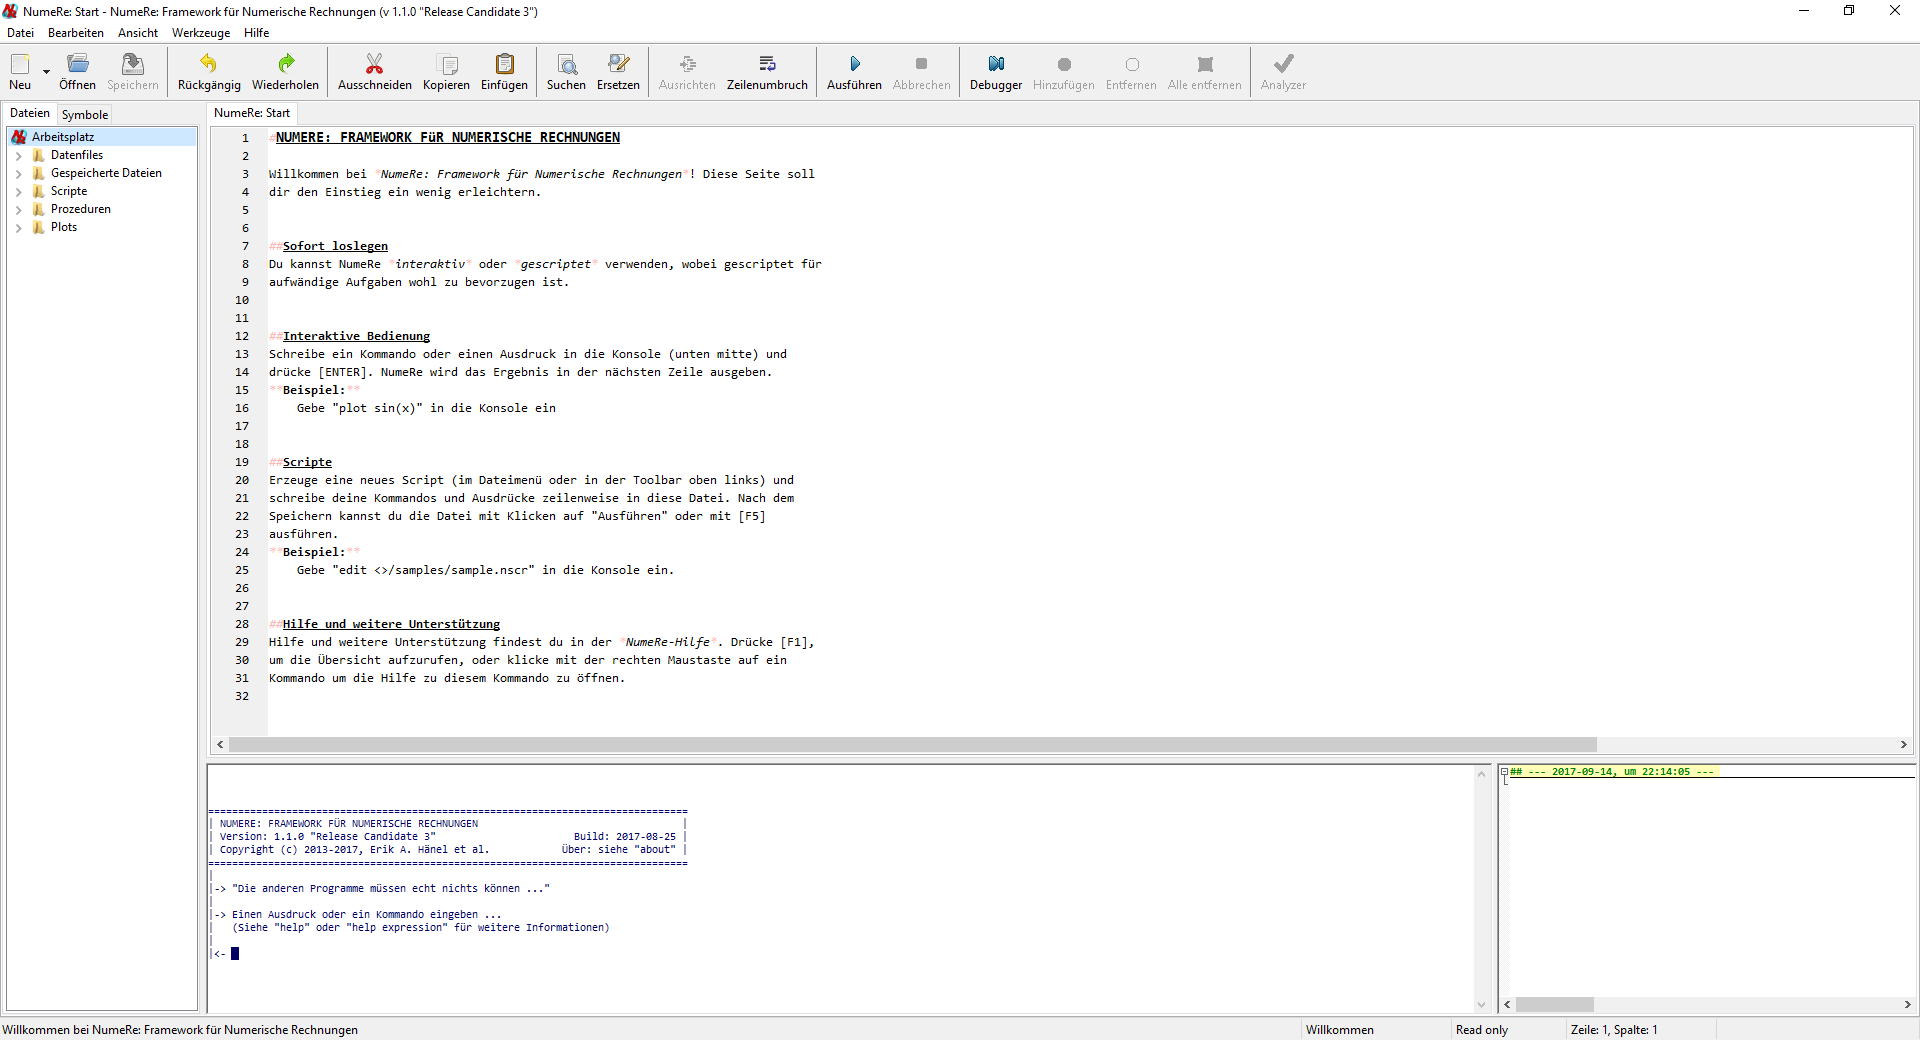
\includegraphics[width=\textwidth]{_graphics/ui.png}
					\caption{The starting view of \NR\ with the described interface elements. The starting page of \NR, which describes some basics, is also visible. \emph{Note: All screenshots shown in this document are in german language but if you've installed the english version, the interface language will be English, of course}}
					\label{fig:ui}
				\end{figure}
				The user interface of \NR\ is separated in five central elements. Most important of them is the \emph{console} (bottom center) and the \emph{editor} (top right). With the console one may interact directly with \NR\ and the editor may be used to edit text files, \NR\ scripts and \NR\ procedures. The \emph{entry history} (bottom right) is an additional element, which protocols all entries in the console, so that they may be repeated by dragging them to the console or by double clicking in them. The \emph{file tree} (left sidebar, first tab) and the \emph{symbol tree} (left sidebar, second tab) support the navigation in the files or the commands and functions, respectively. The editor itself also contains tabs, so that multiple files may be opened and edited.
				
				During the first start the \NR\ editor displays a starting page, which shall make the first task in the application more easy. Users, which are already knowing similar software (such as \textsc{Matlab}), will get familiar with these information really fast. However, we will add some first words.
				\begin{figure}[p]%
					\centering
					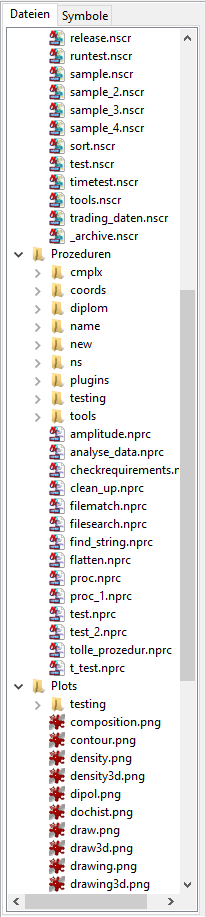
\includegraphics[width=0.2\textwidth]{_graphics/filetree.png}\hspace{5em}
					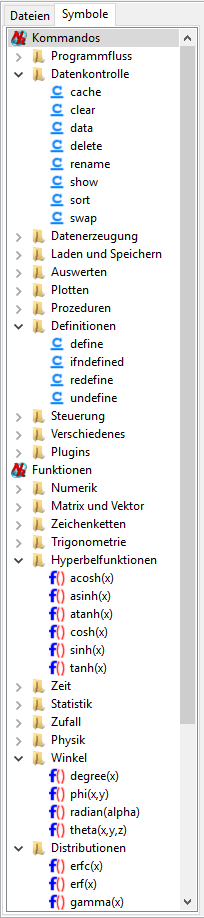
\includegraphics[width=0.2\textwidth]{_graphics/symboltree.png}
					\caption{File and symbol tree in the \NR\ interface}
					\label{fig:trees}
				\end{figure}
				
				First, we'll look at the interaction over the console. There's an arrow \lstinline+<-+ at the beginning of the line, which emphasises that an input is expected (\autoref{fig:ui}). The program's output is prefixed with an arrow, pointing in the opposite direction \lstinline+->+. You may \emph{only} enter something, if such an input arrow (or an explicit claim) appears.
				
				You may enter mathematical-numerical expressions as well as commands into the \NR\ console. The syntax of the mathematical-numerical expressions is quite intuitive and will be described in the next section. The syntax of the commands has to be described more precisely.
				
				We tried to create \NR\ as intuitive as possible. This target should apply to the command syntax as well, but because \NR\ is a long-term and somehow >>grown<< application, we could not fulfill the target everywhere. However, all commands are following the same scheme:
				\begin{verbatim}
					COMMAND [EXPRESSION] [-PARAMETER[=VALUE] [OPTIONS[=VALUE]]]
				\end{verbatim}
				Syntax elements in brackets are sometimes optional or for some commands not present, respectively. Examples for the command syntax are
				\begin{lstlisting}
help
help expression
plot sin(x)
mesh sin(x)+cos(y) -set box
copy <>/samples/data* -target=<loadpath>/*
				\end{lstlisting}
				You'll recognize that (some) commands are not requiring an expression or a parameter.
				
				This command syntax is illustrated in the following sentence:
				\begin{quotation}
					\noindent\emph{>>Apply an action [on something] by using the follwing parameters.<<}
				\end{quotation}
				Applied to one of the upper examples, you can possibly say
				\begin{quotation}
					\noindent\emph{>>Open the documentation article, which has >>expression<< as topic.<<}
				\end{quotation}
				or
				\begin{quotation}
					\noindent\emph{>>Create a meshgrid plot of the function >>sin(x)+cos(y)<< by using the surrounding box.<<}
				\end{quotation}
				
				\helpidx{syntax}
				All commands are listed in the symbol tree and separated in different categories, so that the needed command may be found easily. If you dwell your mouse over a command, a tooltip will be displayed showing a short explanation. If this information is not enough, you may display the documentation article concerning the command, e.g. through\cmd{help}
				\begin{lstlisting}
help plot
				\end{lstlisting}
				All parameters and syntax information for correct execution are listed in these articles, as well as an example of the syntax.
				
				\helpidx{numere}
				If an entry is probably erroneous, \NR\ will display an corresponding message in the console. If a mathematical-numerical expression is erroneous, the position of the error---if possible---will be displayed as well. If the error results from the command syntax, \NR\ will display also a reference to the corresponding article in the \NR\ documentation.
				
				Errors in expressions or commands will abort all calculations. As a consequence all \NR\ scripts and \NR\ procedures will be aborted with an corresponding message as well.
			\section{Preferences}
				All preferences for \NR\ are set in the options dialogue, which may be found in the tools menu. Some settings may additionally be changed with the command \lstinline+set+. The desired setting and its new value have to follow this command:\cmd{set}
				\begin{lstlisting}
set -SETTING=VALUE
				\end{lstlisting}
				If the value of the setting shall contain whitespaces (e.g. a file path), it has to be passed surrounded with quotation marks:
				\begin{lstlisting}
set -SETTING="VALUE WITH WHITESPACES"
				\end{lstlisting}
				The command \lstinline+list+ may display a list of all preferences:\cmd{list}
				\begin{lstlisting}
list -settings
				\end{lstlisting}
				Changed settings are saved at application termination and available again after a restart.
			\section{Simple Calculations}
				As a framework for numerical calculations, \NR\ may of course calculate numerically. The equations, which shall be evaluated, may be entered similar to a pocket calculator. Spaces between operators and values don't play any role, but there are \emph{no spaces} allowed between function names and their argument parentheses. Lower- and uppercase letters are of course different and the multiplication dot \lstinline+*+ mustn't be omitted:
				\begin{lstlisting}
5*cos(_2pi)
				\end{lstlisting}
				multiplies $\cos2\pi$ with 5 and returns the result in the next line. The value \lstinline+_2pi+ is a built-in constant for $2\pi$ and \lstinline+cos()+ is of course the cosine function.

				The built-in constants and functions may be found in the symbol tree. They may be found as well by entering 
				\begin{lstlisting}
list -const
list -func
				\end{lstlisting}
				into the console. \lstinline+list -func+ may also be restricted further.
				
				\helpidx{list}
				\NR\ cannot only handle numbers but also variables. The variables \lstinline+x+, \lstinline+y+, \lstinline+z+, \lstinline+t+ and \lstinline+ans+ are already predefined. However, you may define more variables for the current session. This is done either automatically (if \NR\ stumbles upon an unknown variable) or through and explicit assignment:
				\begin{lstlisting}
neue_variable = 5
				\end{lstlisting}
				(\emph{This variable's name is german for staying consistent with the screenshots.}) This line declares the new variable \lstinline+neue_variable+ and assigns the value 5 to it. The upper equation may now be written as follows:
				\begin{lstlisting}
neue_variable*cos(_2pi)
				\end{lstlisting}
				
				\NR\ may as well evaluate multiple expressions simultaneous. The expressions have to be separated by a comma \lstinline+,+. In the whole (multiple) expression line, \NR\ will evaluate the values from left to right. The line
				\begin{lstlisting}
neue_variable = 5, neue_variable*cos(_2pi), neue_variable = 1
				\end{lstlisting}
				assigns 5 to \lstinline+neue_variable+, calculates $5\cos2\pi$ and finally assigns 1 to \lstinline+neue_variable+ (\autoref{fig:first_calc_1}). This way of writing a calculation may be speed up the evaluation inside of loops significantly.
				
				\helpidx{expression}
				\begin{figure}[htb]%
					\centering
					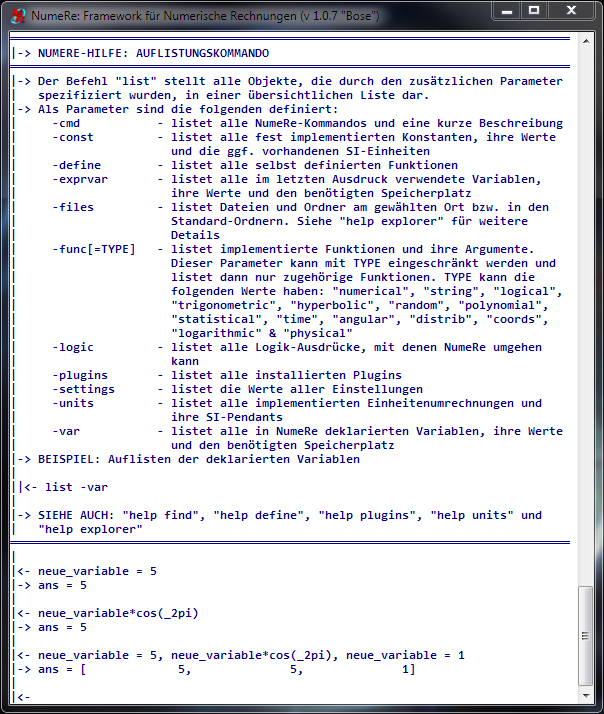
\includegraphics[width=\textwidth]{_graphics/first_calc_1.png}
					\caption{\NR\ after the evalution of the last calculation. You may notice that the input is as well stored in the entry history}
					\label{fig:first_calc_1}
				\end{figure}
			\section{Important Commands}
				You will interact with \NR\ mainly with commands. The most important commands are\cmd{help\\find\\list\\quit}
					\begin{lstlisting}
help
help TOPIC
find TERMS
list -OBJECT
					\end{lstlisting}
					These commands call the integrated documentation (\lstinline+help+ or \lstinline+help TOPIC+ for the desired topic, respectively), the keyword search (\lstinline+find TERMS+) and list objects (\lstinline+list -OBJECT+).
					
					All commands have an entry in the \NR\ documentation. This article may be read by entering \lstinline+help COMMAND+ into the console or by using the corresponding item in the context menu and contains all necessary information about the command and---if applicable---references to further important articles. In the case that an information may not be found direclty in the \NR\ documentation, you may use the keyword search (\lstinline+find+), which will also return the corresponding articles in the \NR\ documentation.
					\paragraph{Note}
						By using a semicolon >>\lstinline+;+<< you may also enter multiple commands and expressions, which shall be evaluated successively, in a single line:
						\begin{lstlisting}
COMMAND1; COMMAND2; EXPRESSION1; COMMAND3; EXPRESSION2; ...
						\end{lstlisting}
		\chapter{Loading and Using Data}
			One of the main tasks in scientific work is data analysis. Therefore it is necessary to use applications, which may load and process the corresponding large amout of data in a reasonable time frame. \NR\ transforms all read data into a table and may calculate statistics, histograms and more elaborate evaluations.
			\section{File Types}
				In addition to simple text files in ANSI format (using the file extensions *.txt and *-dat) \NR\ can load the following file formats:
				\begin{itemize}
					\item \textbf{CassyLab file (*.labx).} This file type is only used by CassyLab and contains a complete CassyLab experiment. However, \NR\ will only extract the data table.
					\item \textbf{CSV file (*.csv).} Comma-Separated-Values files are a nearly-standard for data exchange. However, there is no real >>CSV standard<< defined, so that though tested it is possible that \NR\ cannot read single CSV files correctly. (Please notify the programmer if you face such a problem and forward him the file.)
					\item \textbf{JCAMP-DX file (*.dx, *.jdx and *.jcm).} JCAMP-DX files (meaning \emph{Joint Committee on Atomic and Molecular Physical data -- Data eXchange}) are a standard for file exchanges of spectroscopy data. \NR\ will only extract the data table out of these files.
					\item \textbf{OpenDocument spreadsheet (*.ods).} These are data tables, which are created for example by OpenOffice Calc. \NR\ can only extract the real numerical and string values but not the equations. Please note also that files opened with OpenOffice Calc are locked: these spreadsheets are not readable by \NR.
					\item \textbf{Excel workbooks (*.xls and *.xlsx).} These are data tables, whcich are created by Excel. \NR\ will only extract the numerical and string values, not the equations. The legacy Excel format also doesn't provide the values calculated by the equations in the data tables, so that these are not available in this case. Please note also that files opened with Excel are locked: these workbooks are not readable by \NR.
					\item \textbf{IGOR Binary Waves (*.ibw).} IGOR Binary Waves contain the data of a (1, 2 or 3 dimensional) IGOR wave.
					\item \textbf{NumeRe data file (*.ndat).} NumeRe data files are a data format by \NR, which is used for fast saving and loading of data sets.
				\end{itemize}
				
				\helpidx{load}
				However, \NR\ may not write all of these formats. The following output formats are available:
				\begin{itemize}
					\item \textbf{Text file (*.dat or *.txt).} \NR\ creates a text file in ANSI encoding, which is following the formatting standards in the next section. Most of the other applications should be able to read these files
					\item \textbf{NumeRe  data file (*.ndat).} This file format can only be read by \NR. However, this file format is documented online and may implemented in other programs.
					\item \textbf{CSV file (*.csv).} \NR\ creates a CSV file, where commas \lstinline+,+ are used as column and dots lstinline+.+ are used as decimal separators. (Some table calculations, especially those, which are using the comma as decimal separator, probably cannot read these files: if you replace the commas with semicolons \lstinline+;+ and the dots with commas, this problem should be fixed. The programmer does not understand this behavior.)
					\item \textbf{Excel Workbook (*.xls).} \NR\ may write the data in the legacy Excel-(97-2003)-Format (*.xls) for further processing in Excel and similar applications.
					\item \textbf{\TeX\ file (*.tex).} \NR\ writes a table using the \TeX\ standard. The comments in this file contain the preconditions for including the table in a \TeX\ document (\emph{booktabs} and \emph{longtable} Packages).
				\end{itemize}
				
				\helpidx{save}
			\section{Formatting of Text Files}
				Although \NR\ uses the dot \lstinline+.+ in the console as decimal separator, it is not necessary for files. \NR\ may even read files, which are using the comma and the dot mixed. All commas are transformed to dots internally.
				
				However, text files have to be formatted as a table. It is not relevant, if the columns of this file are separated using whitespaces, tabulators or a mixture of both.
				
				If you have text inside of the data table, it will be ignored. If you want to provide a column header, you have to put these headers in the last line before the actual data. Whitespaces in a single column header have to be replaced with underscores \lstinline+_+. If you want to provide some comments in this file, prefix that with a \lstinline+#+ at the beginning of the line (Column headers are found even it they are prefixed with a \lstinline+#+). You may also use a separating line between the column headers and the data table made out of \lstinline+=+.
				\begin{verbatim}
					# COMMENT
					# COMMENT
					# HEAD_1  HEAD_2  HEAD_3 [...]
					# =======================[...]
					   0,225      12       0 [...]
					   0,245    12.5      .5 [...]
				\end{verbatim}
				
				\helpidx{data}
			\section{Loading and Using of Files}
				You may load the file in the previously defined formats, if you drag and drop them on the console, use the corresponding item in the context menu of the file tree and through\cmd{load}
				\begin{lstlisting}
load FILEPATH/FILE.EXT
				\end{lstlisting}
				File paths and file names containing whitespaces have to be surrounded with quotation marks. The exemplary \lstinline+FILEPATH+ may be omitted, if the file is located in the default directory \lstinline+<loadpath>+ (which is---as default---the folder >>data<< in the \NR\ root directory). If the file extension \lstinline+.EXT+ is omitted, \NR\ will use the first file matching to \lstinline+FILE+ and determine the filetype by itself. There is further information on this topic in the \NR\ documentation at \lstinline+help load+.
				
				There are some example files in the subdirectory >>samples<< in a default \NR\ installation. You may load them for example through
				\begin{lstlisting}
load <>/samples/data
				\end{lstlisting}
				The symbol \lstinline+<>+ is a path placeholder, which points to the \NR\ root directory. This line loads the file >>data.dat<< to \NR's memory. The data is now available as a table in the data object \lstinline+data()+ and may be used (It is a coincidence that the file and the data object carry the same name. The data of loaded files is always stored to \lstinline+data()+).
				
				You may display the data table with the command \lstinline+show+:\cmd{show}
				\begin{lstlisting}
show data()
				\end{lstlisting}
				This will display the table in a separate window.
				
				You may access the data in \lstinline+data()+ using the so-called \emph{interval syntax} \lstinline+a:b+ (for values ranging from \lstinline+a+ to \lstinline+b+). This is used to define the column and row ranges, from where the data should be taken. You pass these indices inside of the argument parentheses of \lstinline+data()+:\cmd{data()}
				\begin{lstlisting}
data(3,1)
data(:,1)
data(4:55,4)
data(3,3:)
				\end{lstlisting}
				In these examples a single element is selected (\lstinline+data(3,1)+ for third row and first column), a whole column (\lstinline+data(:,1)+ for all rows in the first column), a subselection of a column (\lstinline+data(4:55,4)+ for fourth to 55th row and fourth column) or a subsection of a row (\lstinline+data(3,3:)+ for third row and third to last column).
				
				You only may extract values using columns or rows inside of calculations, i.e. the interval syntax may only be used for rows or columns. It is not possible to perform calculations using subtables, however, you may use the matrix operations out of a later chapter to achieve this behaviour. However, you may use different elements of \lstinline+data()+ in a single expression:
				\begin{lstlisting}
(cos(data(:,1)) + sin(data(:,2))) * sqrt(data(1,3:))
				\end{lstlisting}
				This expression will return as many elements as the longest interval nominates. There are also functions, which can handle an arbitrary number of elements and calculate a single result:
				\begin{lstlisting}
avg(), cmp(), cnt(), max(), med(), min(), norm(), num(), prd(), std(), sum(), to_char()
				\end{lstlisting}
				These functions calculate statistics of the elements (average, median, standard deviation, minimal and maximal value), summarize or multiply their arguments, search for elements, count elements or transform the values to ASCII character codes (the usage of strings is explained in the part >>Advanced Usage<< and is not relevant at this point).
				
				\paragraph{Note}
					Users, who are already familiar with Matlab or Octave, will know the difference between \lstinline+OPERATOR+ and \lstinline+.OPERATOR+. This doesn't exist in \NR, because \NR\ was completely designed as a table calculation. Elements from different columns or lines will always be processed element by element and not following a matrix or vector algebra (a matrix-matrix or a matrix-vector multiplication is provided by the framework in the context of the \lstinline+matop+ command using the \lstinline+**+ operator).\bigskip\\
				Some commands, like \lstinline+fit+, \lstinline+fft+ and \lstinline+plot+ (and similar) can handle whole subtables. In the context of this commands you may use the interval syntax in both, columns and rows.
				
				The table in \lstinline+data()+ is a so-called \emph{read-only} data set. This means that the data in this table may not be overwritten or modified in other means. In a later chapter we will explain the caches as tables, which may be manipulated.
				
				\helpidx{data}
			\section{Data Analysis}
				The data analysis is probably the main reason, why someone should search for a fast and simple numerics application. \NR\ provides many predefined functions for analysis, which may be used fast and mostly uncomplicated. The needs for the most common statistics should be fulfilled satisfyingly.
				
				You may either calculate the statistics all at once with the command \lstinline+stats+\cmd{stats}
				\begin{lstlisting}
stats data(i1:i2,j1:j2)
				\end{lstlisting}
				or single with the statistical functions, which where mentioned in the previous section:
				\begin{lstlisting}
std(data(i1:i2,j1))
avg(data(i1:i2,j1))
[...]
				\end{lstlisting}
				The command \lstinline+stats+ returns nearly all reasonable statistical value of the table, which is for example the average, the standard deviation and the standard error, RMS, skewness, excess and the student factor (for a two-fold 95 \%\ confidence interval). Most of them can also be calculated through single functions.
				
				\helpidx{stats}
				A very common way of analyzing a data set is generating a histogram. Histograms are a way to visualize the frequency of a measured quantity. This may either be the period of a oscillation, or the life time of elementary particles or another quantity.
				\begin{figure}[htb]%
					\centering
					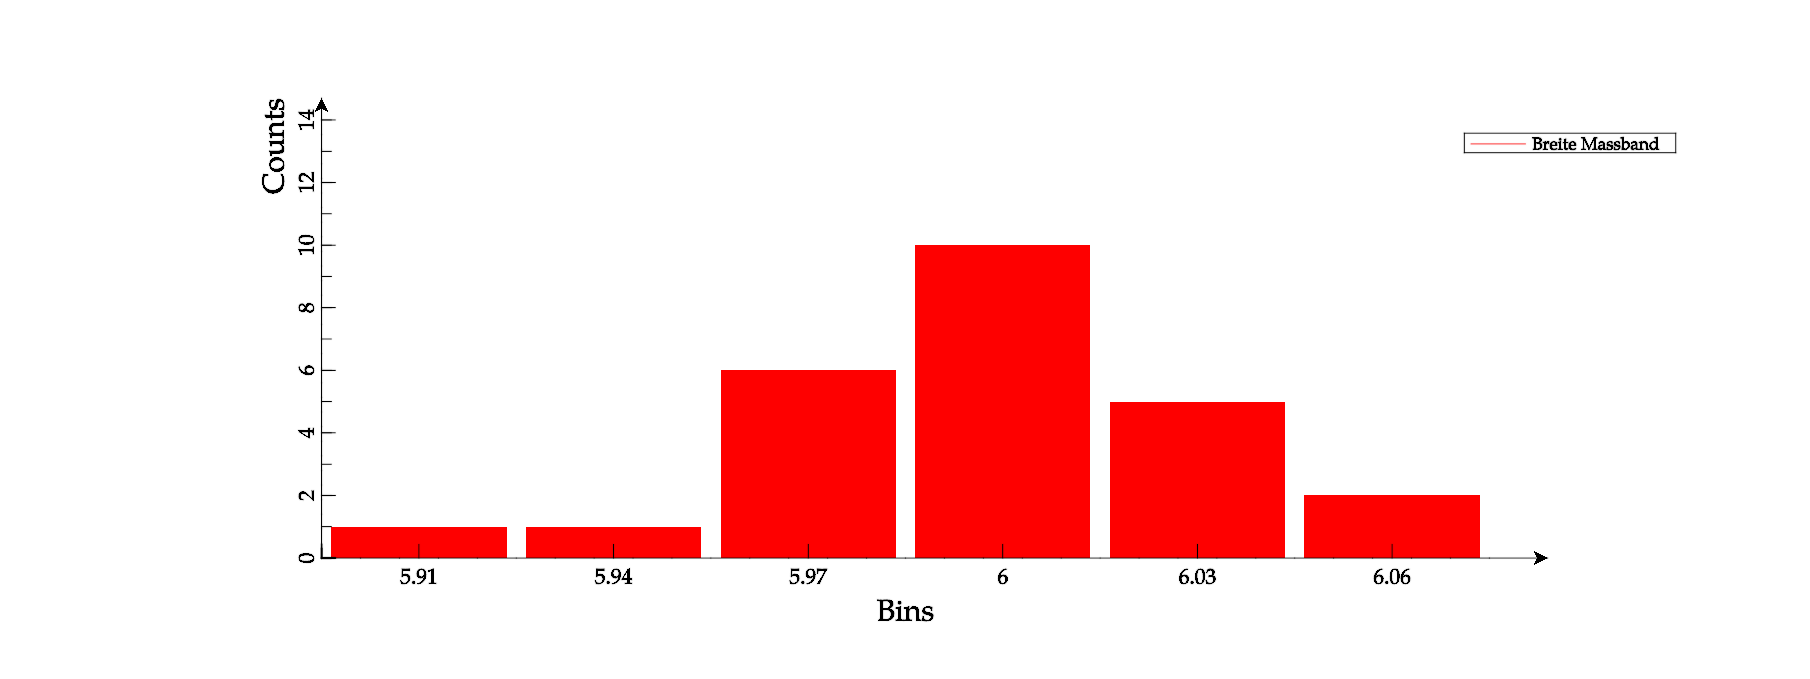
\includegraphics[width=\textwidth]{_graphics/histogramm.png}
					\caption{Histogram of a data set, which was created using \lstinline{hist}}
					\label{fig:histogramm}
				\end{figure}
				
				Histograms of the loaded data are created using \cmd{hist}
				\begin{lstlisting}
hist data(i1:i2,j1:j2)
				\end{lstlisting}
				The command \lstinline+hist+ supports a large number of parameters, which may modify the created histogram even further, though the results without any parameters are already good (\autoref{fig:histogramm}). The number of used bins is determined by the \emph{Rule of Sturges}, but may also be set directly or based upon the \emph{Rule of Scott} or the \emph{Rule of Freedman and Diaconis}.
				
				A histogram is calculated for each column of the data set and the results are presented in a common graph. Columns, which don't contain any reasonale data, have to be excluded using the interval syntax.
				
				\NR\ may also calculate histograms out of a two-dimensional data set. You either have to pass the option \lstinline+grid+ to \lstinline+hist+, then a single histogram of only the $z$ values ignoring their spatial information is calculated. Or you can use the command \cmd{hist2d}\lstinline+hist2d+ for histograms in two spatial directions (like projections along the $x$ and $y$ axes). Further details are listed in the corresponding documentation article.
				
				\helpidx{hist}
				One additional, very common way of analyzing data next to histograms and statistics is to fit a function (sometimes called \emph{model} or \emph{regression curve}) to the measured (and already somehow processed) data.
				
				To fit a function \lstinline+FUNCTION()+ to data in \lstinline+data()+, you can use the command \lstinline+fit+:\cmd{fit}
				\begin{lstlisting}
fit data(:,j1:j2) -with=FUNCTION(x,PARAMS) params=[PARAMS=INITIALW.]
fit data(:,1:2) -with=A*sin(B*x+C) params=[A=1,B=3,C=0]
				\end{lstlisting}
				\NR\ will now try to alter the parameters \lstinline+PARAMS+ in a way that the \lstinline+FUNCTION()+ matches the data points best. The fitted values are stored in the parameters so that you can continue your calculations with these values directly. (In newer \NR\ versions it os not necessary to provide the parameters through \lstinline+params+. \NR\ will detect them on its own.)
				
				If \NR\ reaches an optimal set of parameters, it will cancel the algorithm and return an overview of the parameters, which is presented as an example in the following:
				\begin{verbatim}
					Function: 0.646875*sin(3.00223*x+0.00837336)
					Data points:                            101 without weighting factors
					Degrees of freedom:                     98
					Parameters for the algorithm:           TOL=0.0001, MAXITER=500
					Iterations:                             7
					Weighted sum of the residuals (chi^2):  2.33825
					Variance of the residuals (red. chi^2): 0.0238597
					Standard deviation of the residuals:    0.1544658

					Parameter  Initial value        Fitted        Asymptotic standard error
					-----------------------------------------------------------------------
					A                      1     0.6468754    ± 0.02188576         (3.383%)
					B                      3      3.002228   ± 0.005649476        (0.1882%)
					C                      0   0.008373364    ± 0.06579646         (785.8%)
					----------------------------------------------------------------------

					Correlation matrix of the fitted parameters:

					/          1     0.0159    -0.0164 \
					|     0.0159          1     -0.862 |
					\    -0.0164     -0.862          1 /

					Fitting result analysis:
					The fitted function could describe the trend of the data points, but 
					there is some room for optimisation.
				\end{verbatim}
				This overview contains the important quantity $\chi^2$, which contains the sum of the quadratic deviations of the data points to the fitted function. In addition, you'll find the result values of the parameters and the calculated error values, which may inserted in the concluding error progression. The correlation matrix of the parameters contains an information, how the parameters are connected to each other and the fitting result analysis is a summary of what can be learned from the value of $\chi^2$. This overview will also be stored in the fit log file at \verb+<savepath>/numerefit.log+.
				\begin{figure}[htb]%
					\centering
					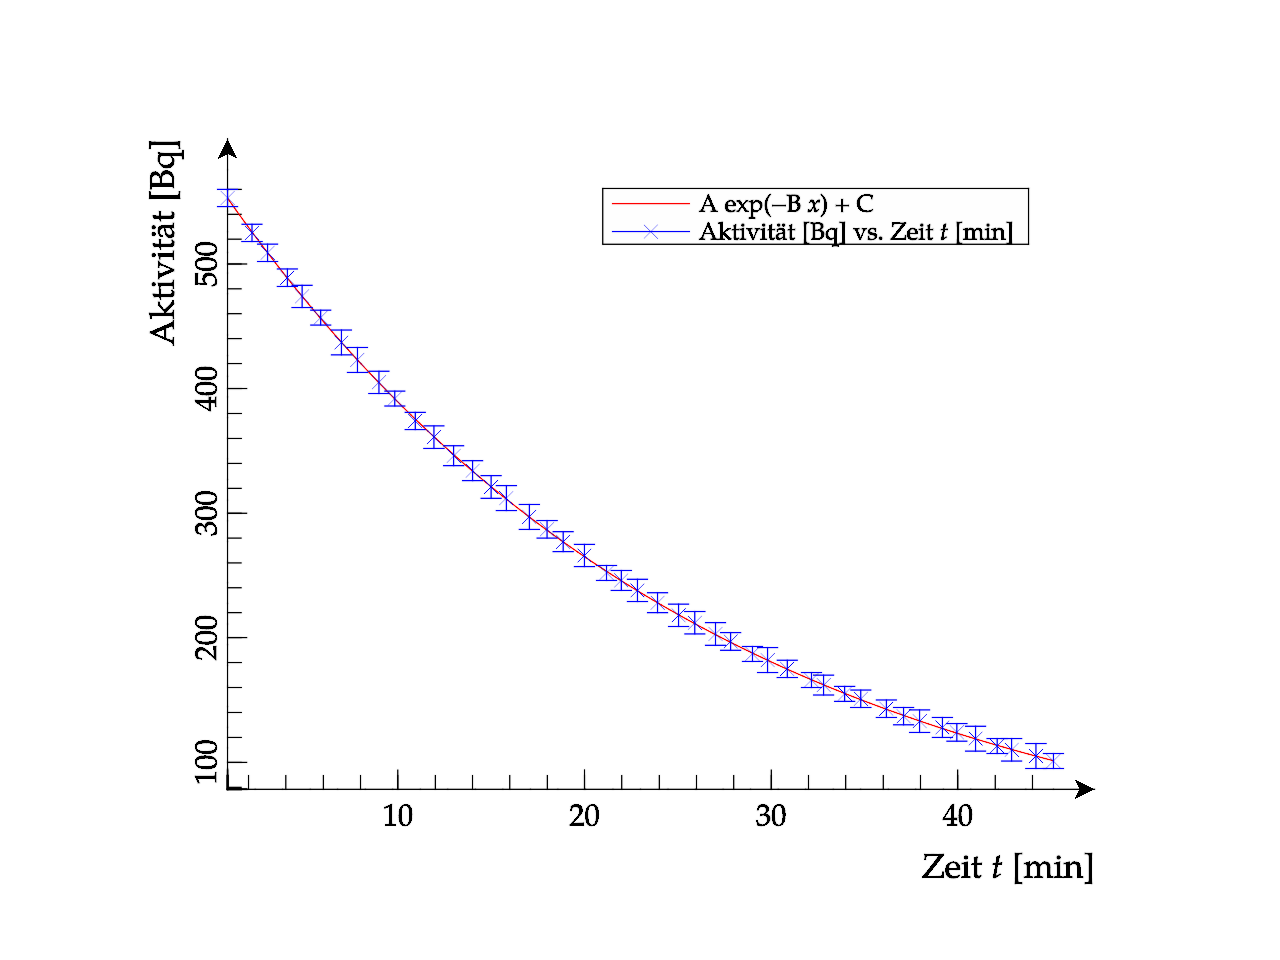
\includegraphics[width=0.8\textwidth]{_graphics/plot.png}
					\caption{Fitting a model for an exponential decay with \lstinline{fitw}}
					\label{fig:fit}
				\end{figure}
				
				\paragraph{Note}
					If the quantity $\chi^2$ is an indicator on the quality of the fit, can be discussed. In common, one assumes that a fit with the smallest possible $\chi^2$ value has the best possible parameter set. More precise: it's the so-called reduced $\chi^2$ value, which is the important quantity: if it is noticeable smaller than 1, the resulting parameter set seems to fit the data points quite well. If you perform a fit, which will consider the error estimations (see below), this value should be in the range of 1. \NR\ will consider all these conditions and return a corresponding fitting result analysis. But note that the analysis may only support and not fully replace the optical comparation of fitted function and data points.\bigskip\\
				After the fitting procedure, the fitted function may be displayed graphically using the command \lstinline+plot+ (see next chapter) (\autoref{fig:fit}). This is a good possibility to check the results of the fitting procedure (and should always be performed).
				
				If you can estimate the measurment errors, \NR\ may consider these values. Just use\cmd{fitw}
				\begin{lstlisting}
fitw data(:,1:2:3) -with=A*sin(B*x+C) params=[A=1,B=1,C=0]
				\end{lstlisting}
				\lstinline+fitw+ (for \emph{weighted fit}) uses the error estimations in the third column to calculate the weighting factors for the data points: data points with higher errors are considered less important than those with small errors.
				
				If a fitting procedure does not converge, it may help varying the initial values of the parameters (which shall be passed everytime). It also may help to restrict the fitting interval. This may be done either through restricting the rows in \lstinline+data()+ or through passing the option \lstinline+x=a:b+:
				\begin{lstlisting}
fit data(:,1:2) -with=A*sin(B*x+C) params=[A=1,B=1,C=0] x=0:4
				\end{lstlisting}
				In addition the maximal number of iterations, the precision and further restrictions of the parameters can be set. The last option may have a large influence on the stability of the algorithm.
				
				\helpidx{fit}
				All mentioned commands are acting along the columns. If the data is organized in rows, one has to perform the following line\cmd{copy}
				\begin{lstlisting}
copy data(:,:) -target=cache(:,:) transpose
				\end{lstlisting}
				and replace \lstinline+data+ with \lstinline+cache+ in all previous examples.
		\chapter{Creating Graphs}
			A very important functionality of \NR\ is the creation of function and data graphs. You may visualize the behaviour of functions and data and analyze them more easy. \NR\ can store all created graphs in image files, if you specify that in the options list of the graph.
			\section{Types of Graphs}
				\NR\ knows a large number of different plot types, which may be modified further by passing further options to the options list. The following list shall only mention the most important plot types. You can get the full list by entering the command \lstinline+list -cmd+:
				\begin{lstlisting}
plot
plot3d
mesh
dens
vect
vect3d
...
				\end{lstlisting}
				\begin{itemize}
					\item \lstinline+plot+: this creates a standard graph, which displays $y$ against $x$. This command is being used, if you want to visualize $\sin x$ or $x^2$.
					\item \lstinline+plot3d+: this command creates a graph on the basis of a 3-dimensional trajectory. A trajectory is calculated from three functions sharing the variable $t$ and visualized three-di\-men\-sion\-al\-ly.
					\item \lstinline+mesh+: a function $z = f(x,y)$ may be displayed with this command. A meshgrid is calculated and displayed three-dimensionally.
					\item \lstinline+dens+: this command visualizes the function $z = f(x,y)$ in contrast to \lstinline+mesh+ only through colour values projected to the $x$-$y$ plane.
					\item \lstinline+vect+: this plotting style calculates a vector plot of a 2D vector field: $\vec A(x,y) = A_x(x,y)\,\hat e_x + A_y(x,y)\,\hat e_y$.
					\item \lstinline+vect3d+: this calculates a vector plot similar to \lstinline+vect+, but it uses a three-dimensional vector field as data basis: $\vec A(x,y,z) = A_x(x,y,z)\,\hat e_x + A_y(x,y,z)\,\hat e_y + A_z(x,y,z)\,\hat e_z$.
				\end{itemize}
			\section{Output}
				The default output channel for plots is the \NR\ GraphViewer, in which the plots may be modified further. Additionally, the plots may be stored into an image file in the PNG format in the directory \lstinline+<plotpath>+ (This is per default the subdirectory >>plots<< in the \NR\ root). You may change the image file format to othe formats. This may be done with the plotoptions \lstinline+opng+, \lstinline+oeps+, \lstinline+ogif+, \lstinline+osvg+ and \lstinline+otex+.
				
				To create a simple plot in for example >>graph\_of\_the\_measurement.png<<, you've to pass the option
				\begin{lstlisting}
opng=graph_of_the_measurement
				\end{lstlisting}
				If the file name of the target file shall contain whitespaces, you've to pass it in enclosing quotation marks.
				
				\helpidx{plotoptions}
			\section{Usage}
				The syntax of all plotting commands is following this scheme:
				\begin{lstlisting}
COMMAND FUNCTIONS/DATA -set OPTIONS
				\end{lstlisting}
				where \lstinline+OPTIONS+ are optional and may be omitted.

				Default variables are $x, y, z$ and $t$. Depending on the actual plotting command, one, two, three or all four of these variables are used as plotting variables and the others are parameters. \lstinline+plot+ uses only $x$, \lstinline+plot3d+ only $t$, \lstinline+mesh+, \lstinline+dens+ and \lstinline+vect+ $x$ and $y$ and \lstinline+vect3d+ uses $x, y$ and $z$. All other variables are parameters.
				
				A simple plot of a sine is created with\cmd{plot}
				\begin{lstlisting}
plot sin(x)
				\end{lstlisting}
				This calculates a sine function from $-10$ to $10$ automatically, where the $y$ axis was chosen fitting but a small amount larger than the minimal and maximal value of the function. The axis labels and the legend are also determined automatically (\autoref{fig:sinusplots}a)
				\begin{figure}[p]%
					\centering
					\subfloat[without options]{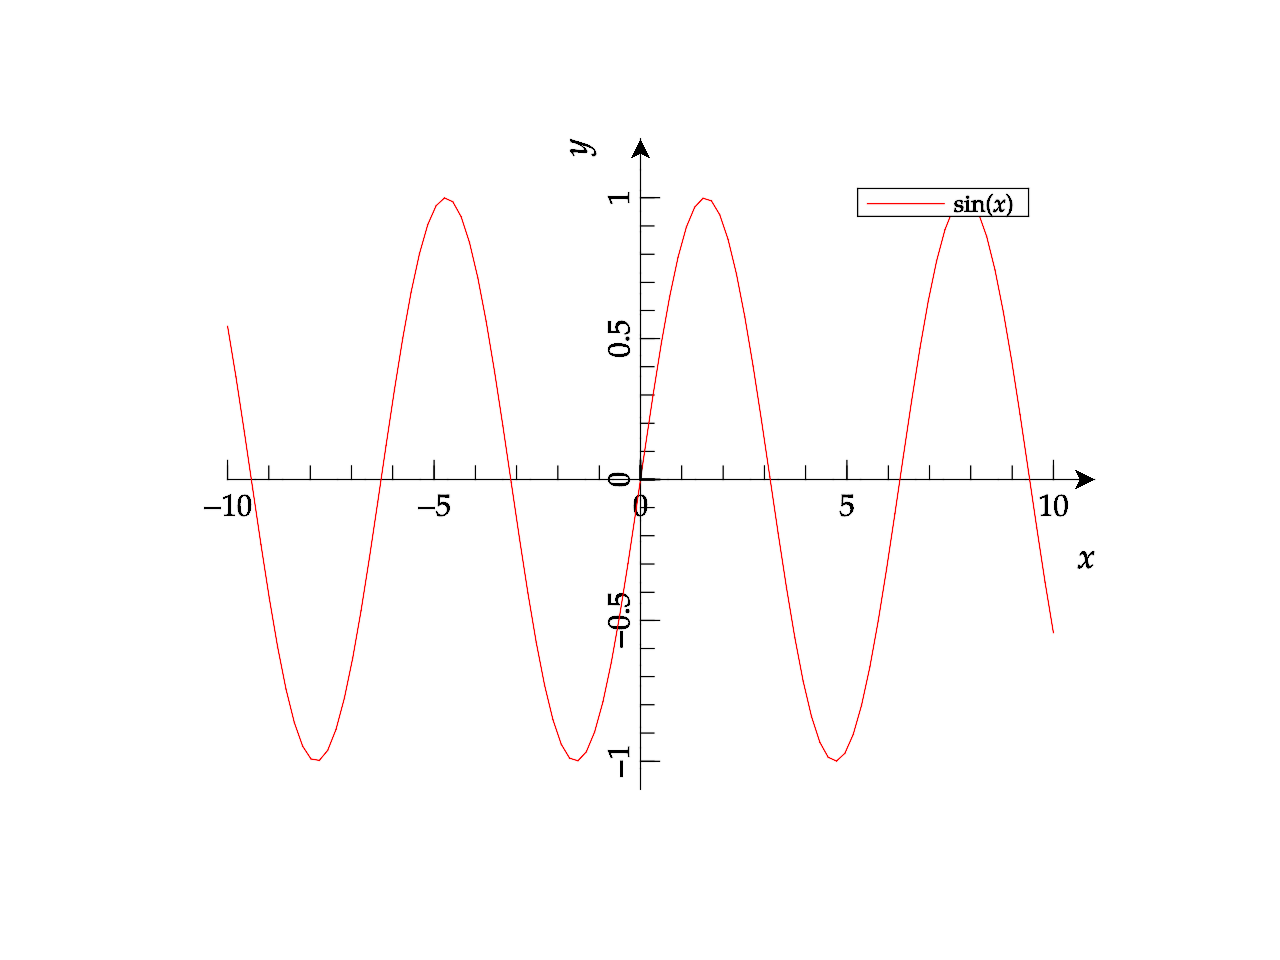
\includegraphics[width=0.45\textwidth]{_graphics/plot_0.png}}
					\subfloat[with \lstinline{box} and \lstinline{grid}]{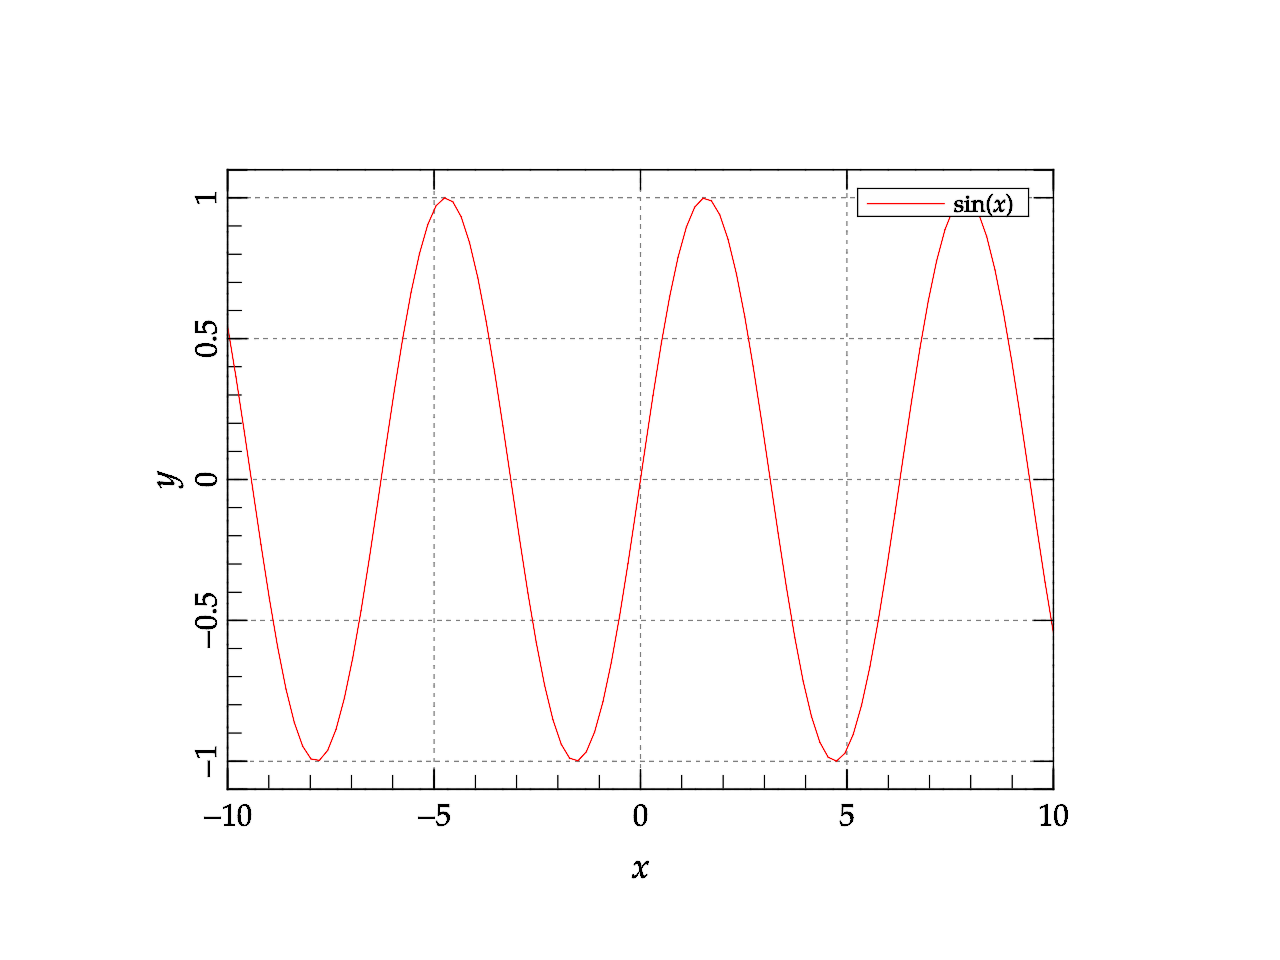
\includegraphics[width=0.45\textwidth]{_graphics/plot_1.png}}\\
					\subfloat[with custom legend]{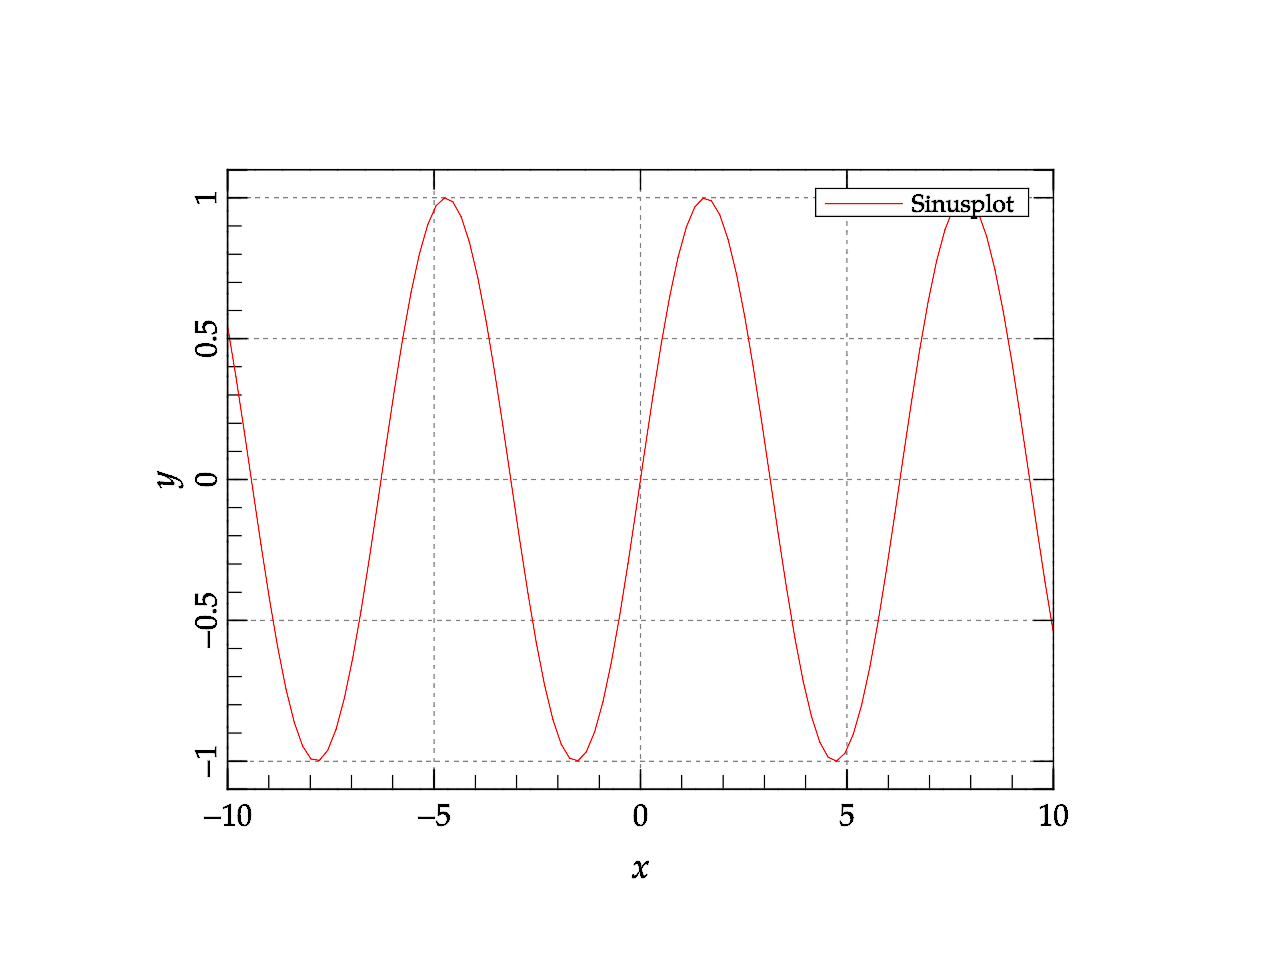
\includegraphics[width=0.45\textwidth]{_graphics/plot_2.png}}
					\subfloat[with data set]{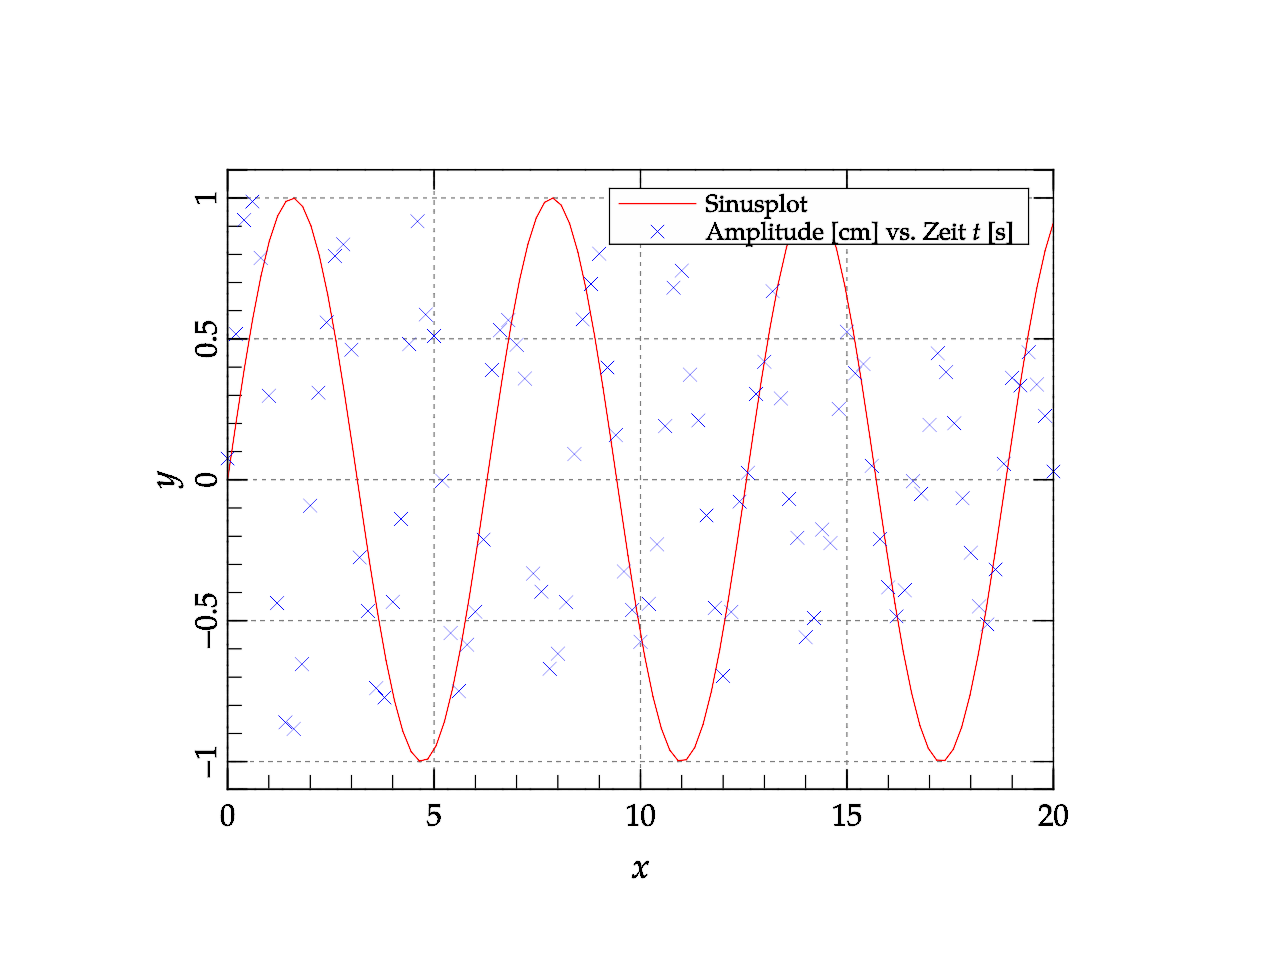
\includegraphics[width=0.45\textwidth]{_graphics/plot_3.png}}\\
					\subfloat[with custom interval]{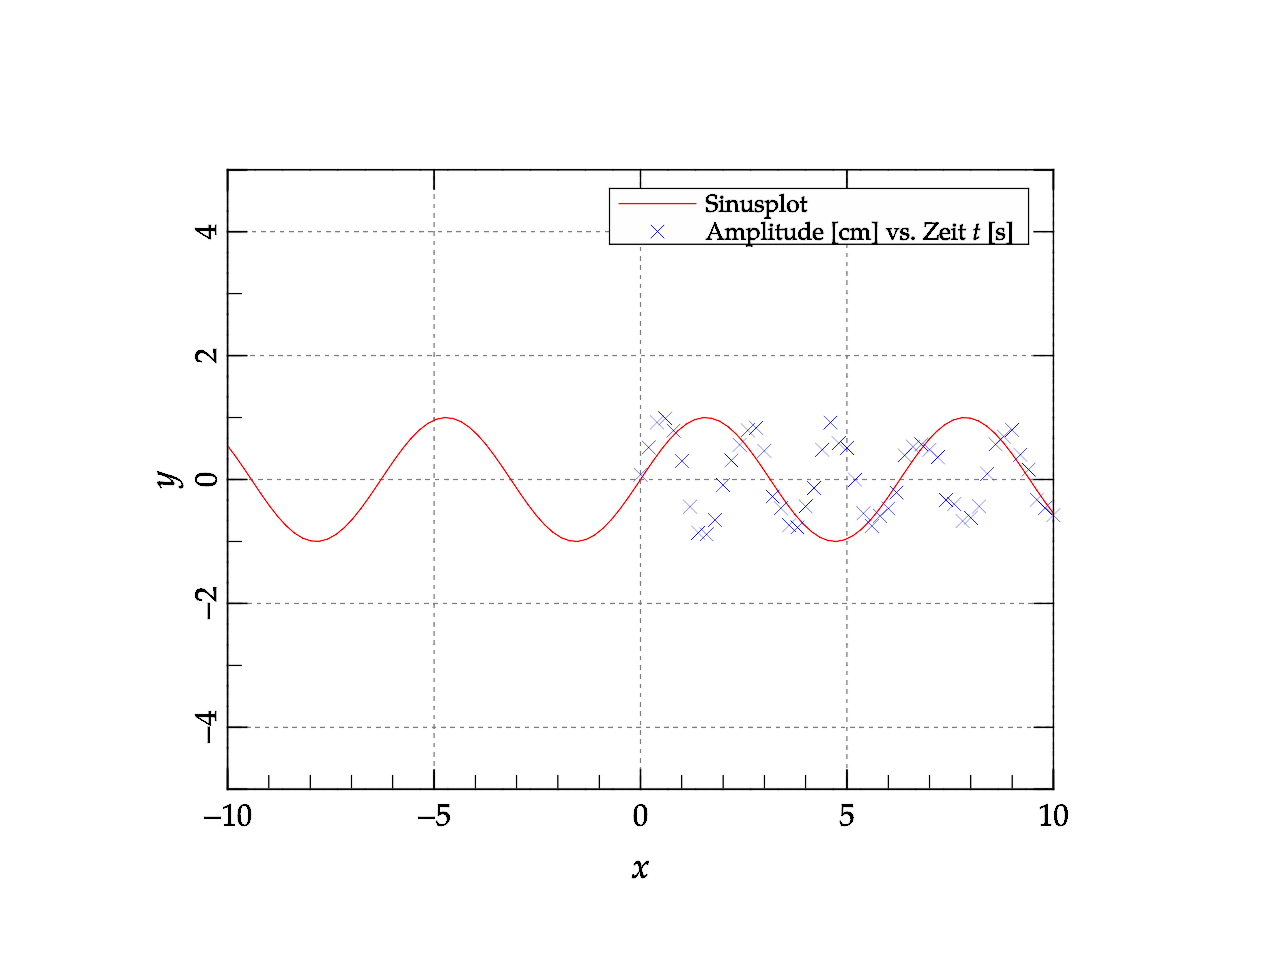
\includegraphics[width=0.45\textwidth]{_graphics/plot_4.png}}
					\subfloat[with errorbars]{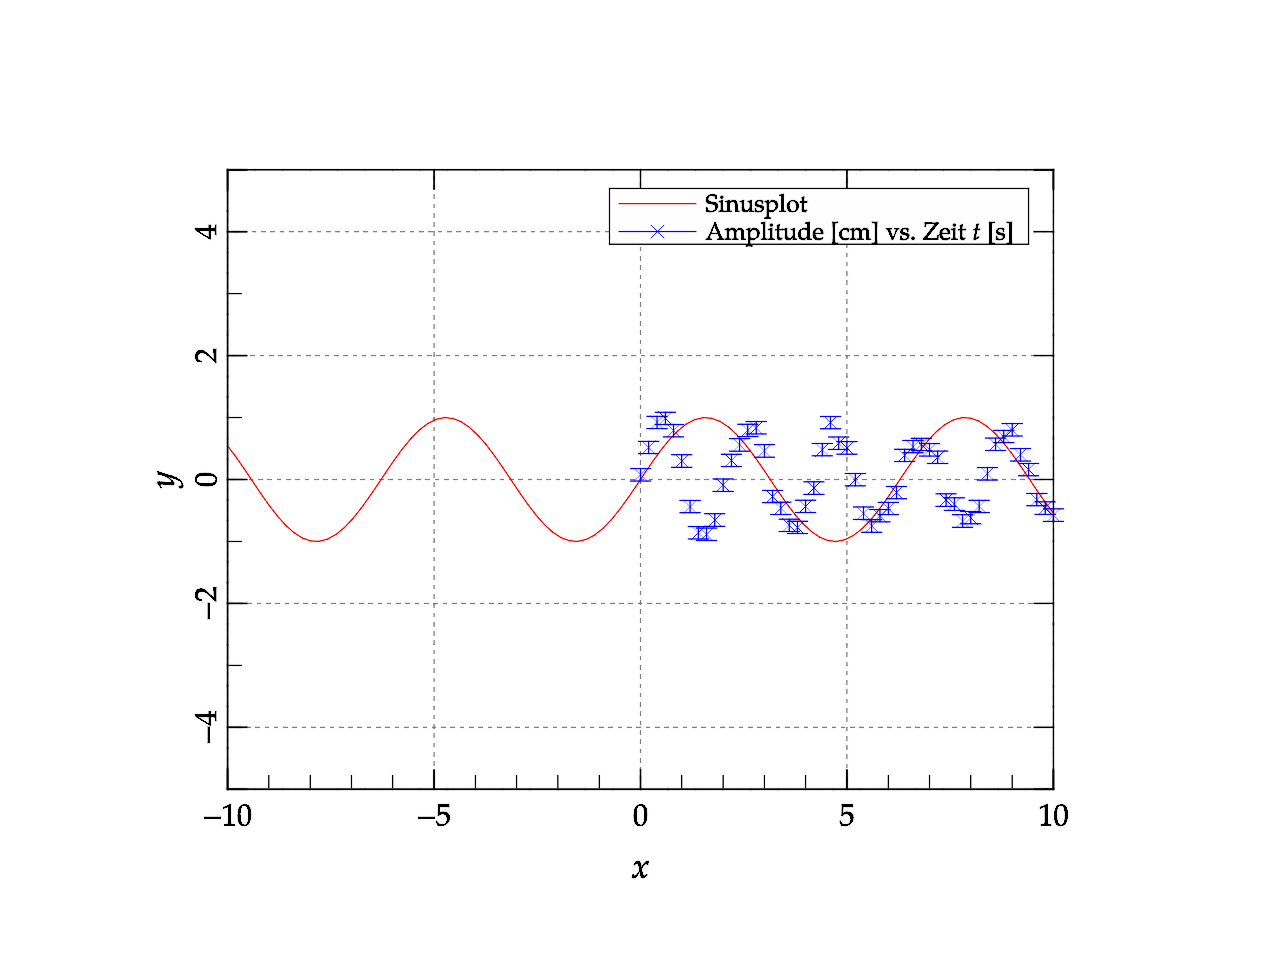
\includegraphics[width=0.45\textwidth]{_graphics/plot_5.png}}
					\caption{The resulting graphs using the shown options}
					\label{fig:sinusplots}
				\end{figure}
				
				\helpidx{plot}
				You are getting a surrounding box and a coordinate grid with 
				\begin{lstlisting}
plot sin(x) -set box grid
				\end{lstlisting}
				This and all further plots will also get a grid and a box (\autoref{fig:sinusplots}b and c).
				
				If you want to have >>Sine function<< instead of >>$\sin(x)$<< as legend, you'll have to enter the following:
				\begin{lstlisting}
plot sin(x) "Sine function" -set box grid
				\end{lstlisting}
				(\autoref{fig:sinusplots}c; An empty legend is achieved by passing an empty string \lstinline+""+)
				
				\NR\ may also display data points graphically. To achieve this, one has to pass the data set in \lstinline+data()+ analogous to a function. If you leave the argument's parentheses empty, this will be replaced automatically with \lstinline+data(:,:)+. You may also specify the desired columns by yourself, e.g. \lstinline+data(:,1:4)+. \NR\ will use either the columns 1 and 4 or the columns 1 to 4, if the corresponding plotting style needs more than two columns. You may specify up to six columns in an arbitrary order: \lstinline+data(:,4:2:6:1:3:8)+.
				
				In combination with the previous example, one may visualize the columns 1 and 2 together with the sine function through
				\begin{lstlisting}
plot sin(x) "Sine function", data() -set box grid
				\end{lstlisting}
				(\autoref{fig:sinusplots}d). Even for \lstinline+data()+ one may pass a customn legend. Otherwise \NR\ will create a combination of the columns titles. Additional it's noticable that adding the data set has scaled the $x$ axis corresponding to the data set. Also noticeable is that \NR\ displays the data points as single points and doesn't connect them with a (non-physical) line.
				
				The plotting intervals may be overwritten for a plot, if they are passed explicitly:
				\begin{lstlisting}
plot sin(x) "Sine function", data() -set box grid [-10:10,-5:5]
				\end{lstlisting}
				This creates a graph with the $x$ interval $[-10;10]$ and the $y$ interval $[-5;5]$ (\autoref{fig:sinusplots}e). This option will \emph{not} be used for successive plots.
				
				Measurements of data points are often combined with measurement errors. If these are known, \NR\ may display them correspondingly. If only the $y$ values have errors, \NR\ needs three columns ($x,y,\Delta y$), if both directions have errors, \NR\ will need four ($x,y,\Delta x, \Delta y$). The needed plotting option is \lstinline+errorbars+ or \lstinline+yerrorbars+, if only $y$ errors are available.
				
				If wie assume that the data points in the upper example have errors in $y$ direction, we may enter:
				\begin{lstlisting}
plot sin(x) "Sine function", data() -set box grid [-10:10,-5:5] yerrorbars
				\end{lstlisting}
				Errorbars in $y$ direction are appearing, although the number of columns was not changed! \NR\ interprets the empty argument's parenthesis now automatically in another way and uses the first three columns (\autoref{fig:sinusplots}f).
				
				\helpidx{plotoptions}
				\cmd{mesh}In another case a two-dimensional function shall be visualized using a meshgrid plot: the function is the cardinal sine of $\varrho$ ($\text{sinc}\,\varrho$):
				\begin{lstlisting}
mesh sinc(norm(x,y))
				\end{lstlisting}
				\begin{figure}[p]%
					\centering
					\subfloat[only \lstinline{mesh}]{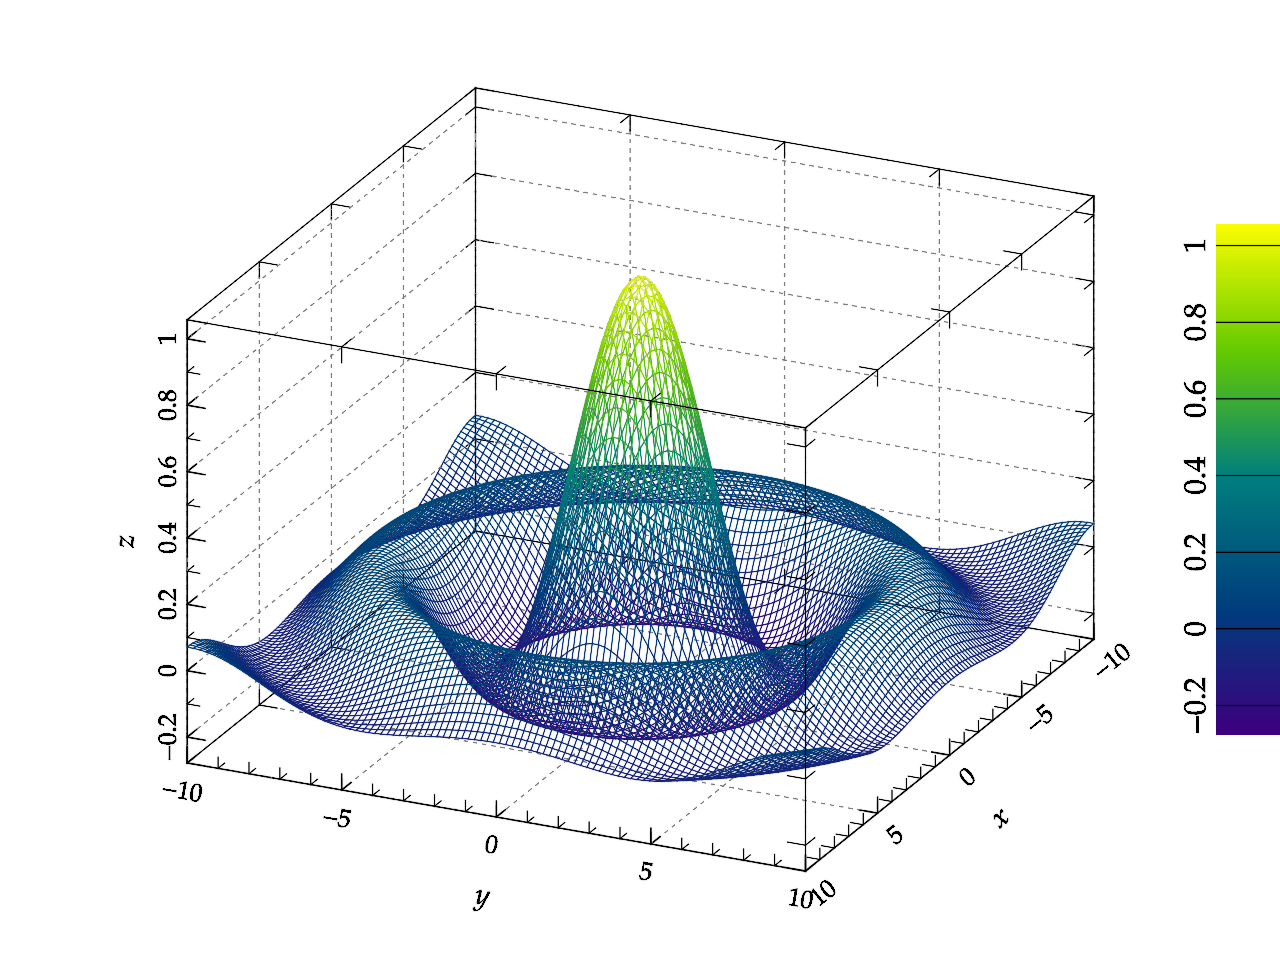
\includegraphics[width=0.45\textwidth]{_graphics/mesh_0.png}}
					\subfloat[with \lstinline{nobox}]{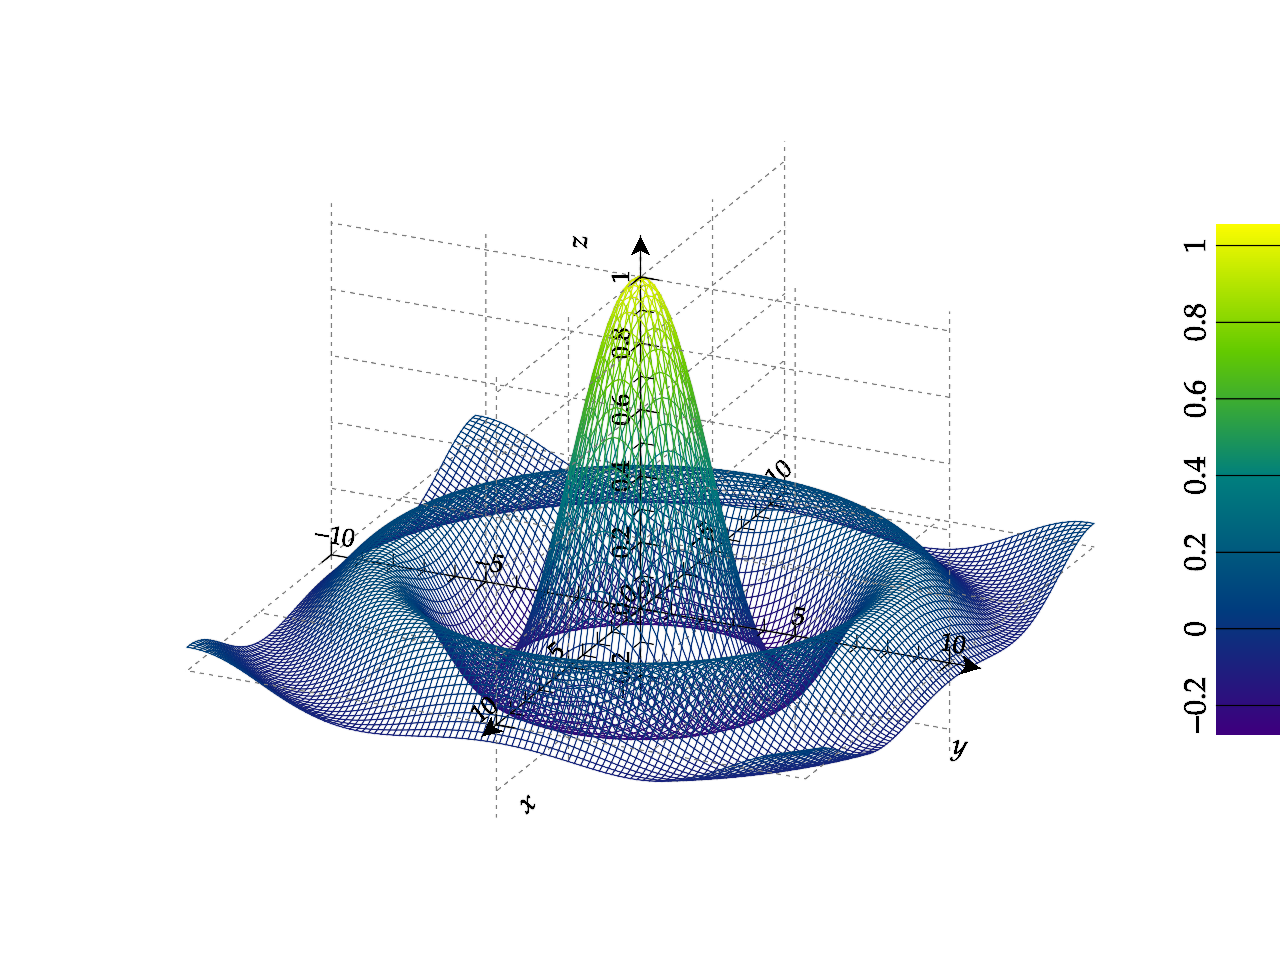
\includegraphics[width=0.45\textwidth]{_graphics/mesh_1.png}}\\
					\subfloat[with \lstinline{rotate}]{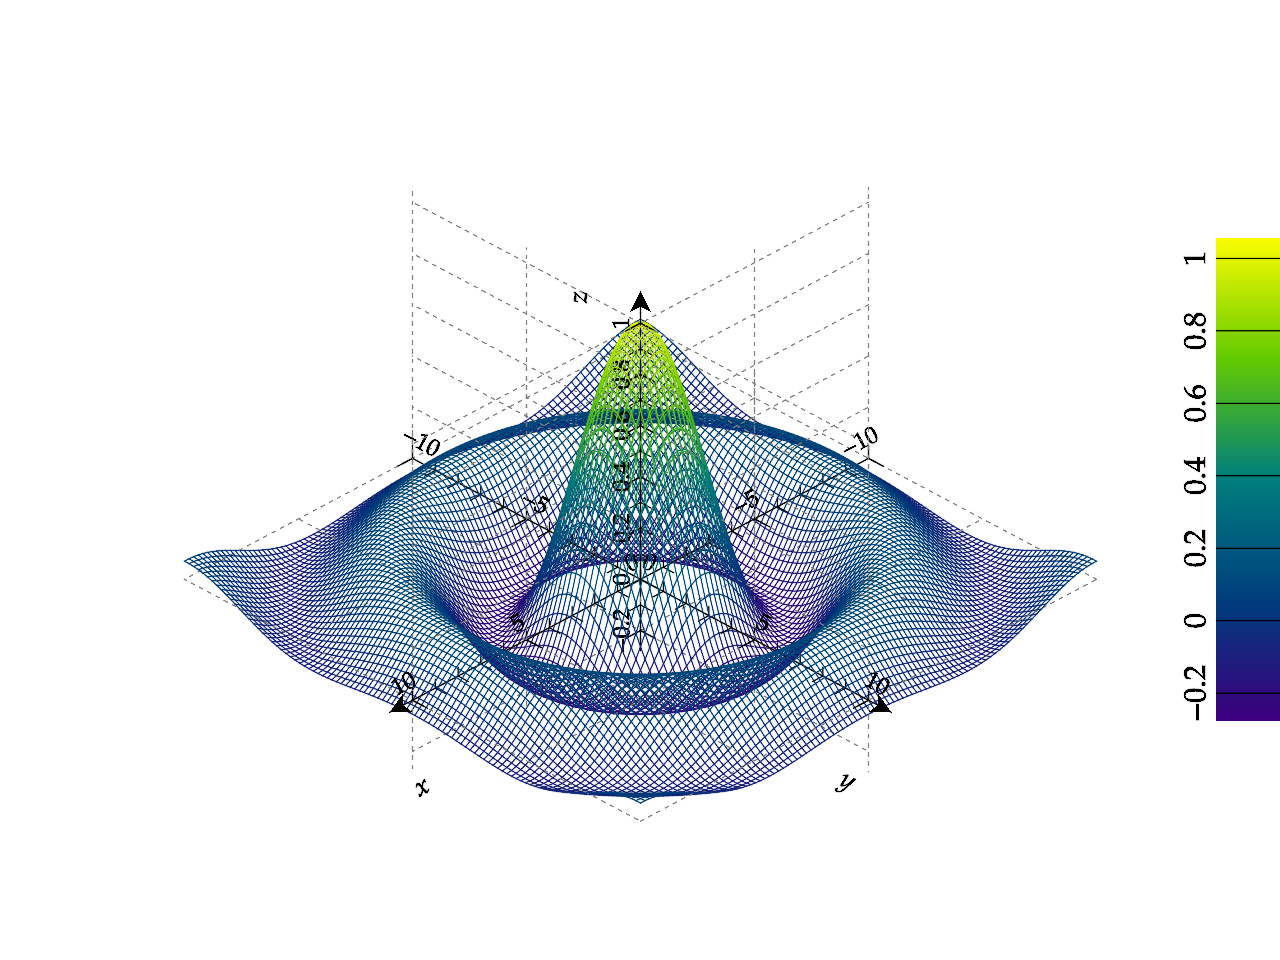
\includegraphics[width=0.45\textwidth]{_graphics/mesh_2.png}}\\
					\subfloat[only \lstinline{vect}]{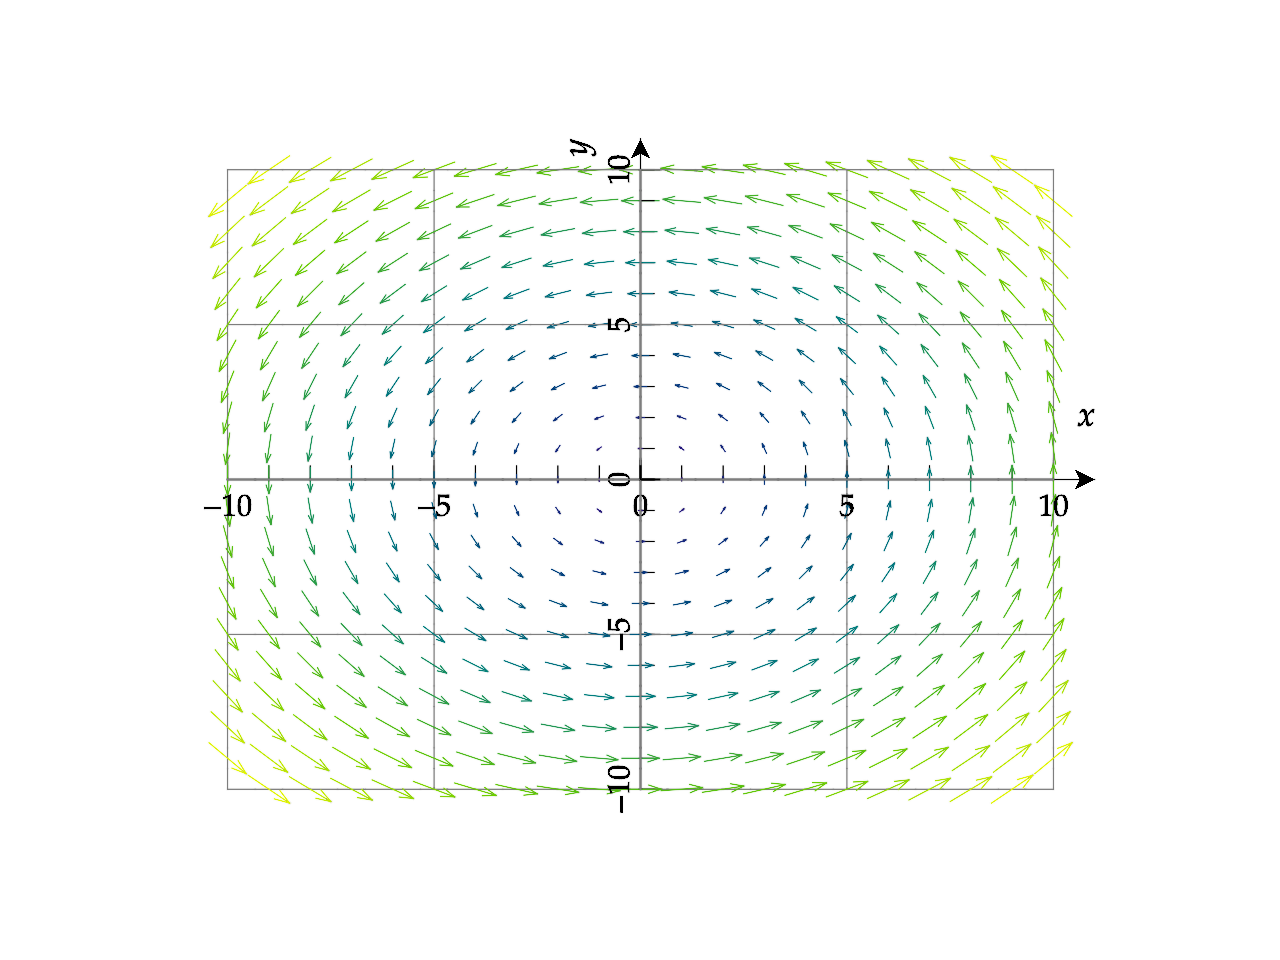
\includegraphics[width=0.45\textwidth]{_graphics/vect_0.png}}
					\subfloat[with \lstinline{flength}]{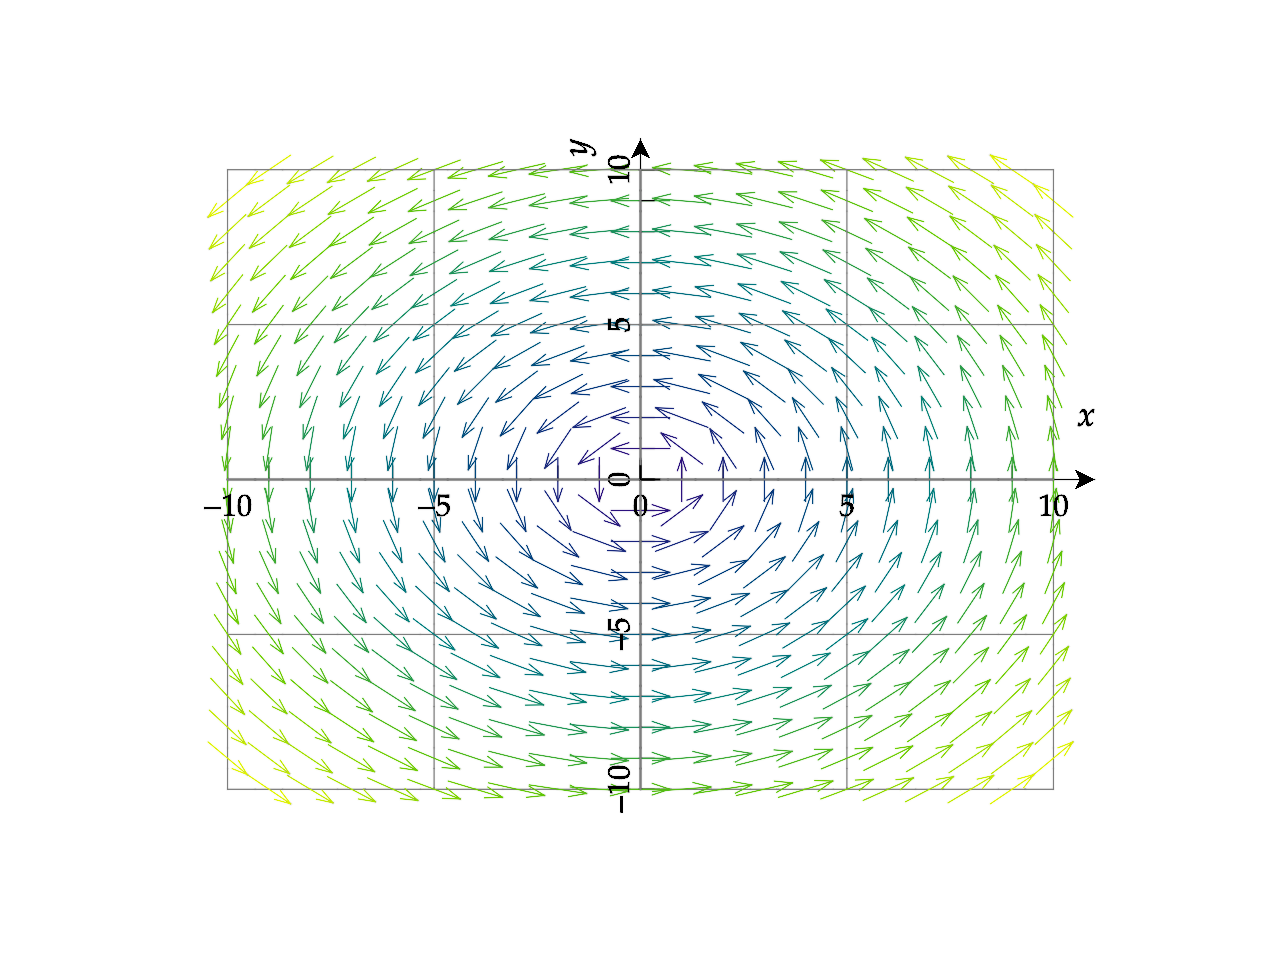
\includegraphics[width=0.45\textwidth]{_graphics/vect_1.png}}
					\caption{Results of the meshgrid and vector plots}
					\label{fig:mesh_vect}
				\end{figure}
				The command \lstinline+mesh+ creates the desired meshgrid plot (\autoref{fig:mesh_vect}a). The function \lstinline+norm()+ is the $n$-dimensional, euklidic vector norm (This function will accept an arbitrary number of arguments):
				\begin{equation*}
					\text{norm}(x,y,z,\ldots) := \sqrt{x^2+y^2+z^2+\ldots}
				\end{equation*}
				In this case $\text{norm}(x,y) = \varrho$. Because this was visualized directly after the previous plots in this chapter, you should notice that the meshgrid plot is also surrounded by a box and has a grid in the background. To remove the box, you may enter \lstinline+nobox+ (\autoref{fig:mesh_vect}b):
				\begin{lstlisting}
mesh sinc(norm(x,y)) -set nobox
				\end{lstlisting}
				
				The meshgrid plot is oriented automatically into a predefined direction. This may also be changed:
				\begin{lstlisting}
mesh sinc(norm(x,y)) -set rotate=45,135
				\end{lstlisting}
				The graph now appears now more tilted and the $x$ and $y$ axes seem to be symmetric to both sides (\autoref{fig:mesh_vect}c). You probably notice that the graph was oriented with these angular values into the direction of the first space diagonal. The angular values of \lstinline+rotate+ have to be passed in degrees in the order $\vartheta,\varphi$, where $\vartheta$ tilts the graph and $\varphi$ rotates it.
				
				\helpidx{mesh}
				A further example is the vectorfield plot of a two-dimensional rotation field:
				\[\vec A(x,y) = 2\svec{-y\\x}\]
				This is achieved through\cmd{vect}
				\begin{lstlisting}
vect -2*y,2*x
				\end{lstlisting}
				The first function will be interpreted as the amplitude in $\hat e_x$ direction and the second in $\hat e_y$ direction (\autoref{fig:mesh_vect}d). This command will only accept only one vectorfield per plot.
				
				The length of the vector arrows correspond to the local amplitude of the vectorfield. To deactivate this effect, you may pass
				\begin{lstlisting}
vect -2*y,2*x -set flength
				\end{lstlisting}
				(\autoref{fig:mesh_vect}e).
				
				\helpidx{vect}
			\section{Coordinate Systems}
				The last section of this chapter shall focus on the different coordinate systems. \NR\ supports three different coordinate systems: the \emph{cartesian}, the \emph{polar} or \emph{cylindrical} and the \emph{spherical} one.
				\begin{figure}[htb]%
					\centering
					\subfloat[\lstinline{plot} with \lstinline{coords=polar}]{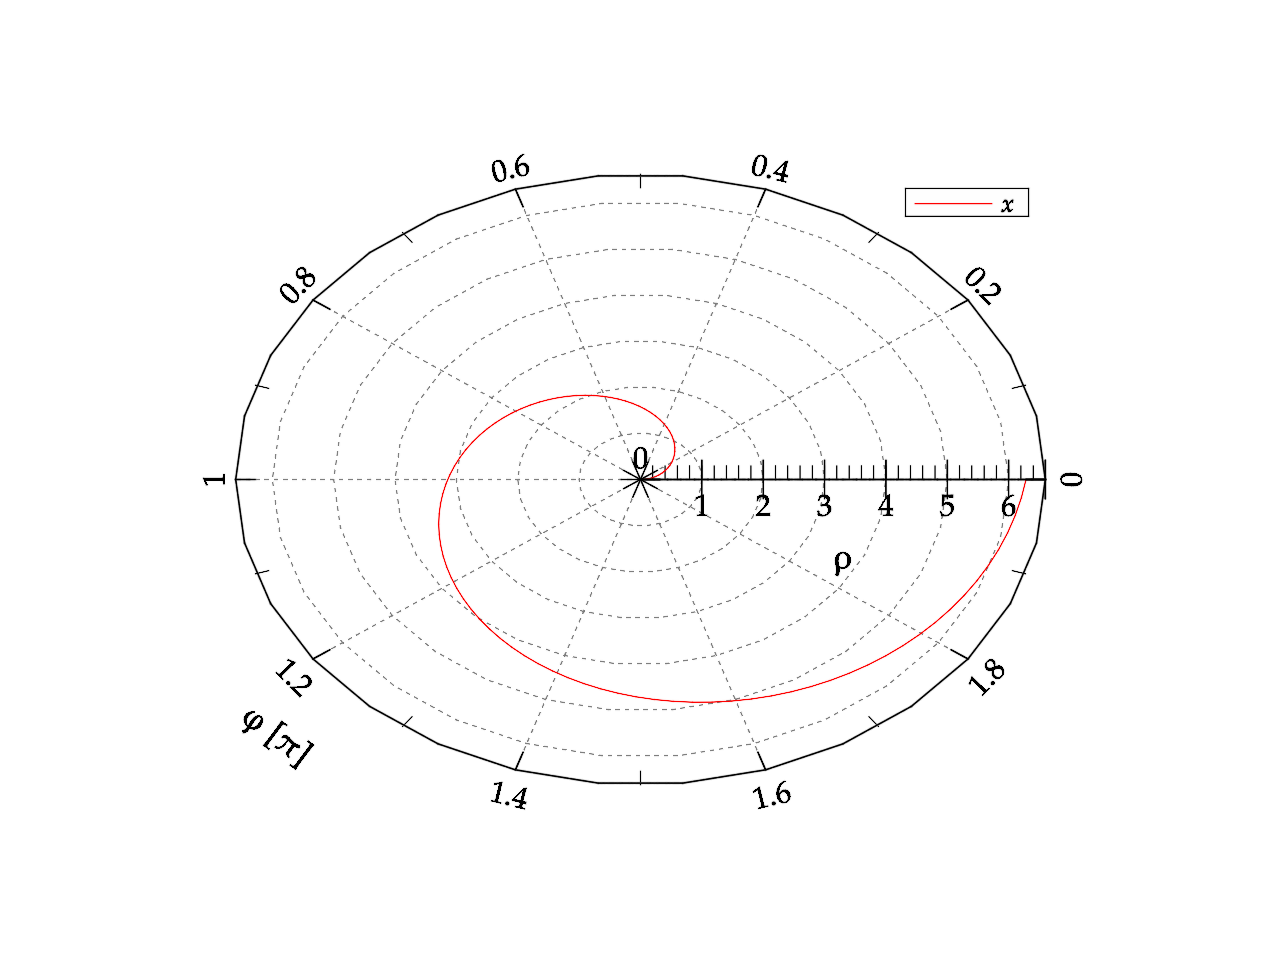
\includegraphics[width=0.45\textwidth]{_graphics/plot_6.png}}
					\subfloat[with larger interval]{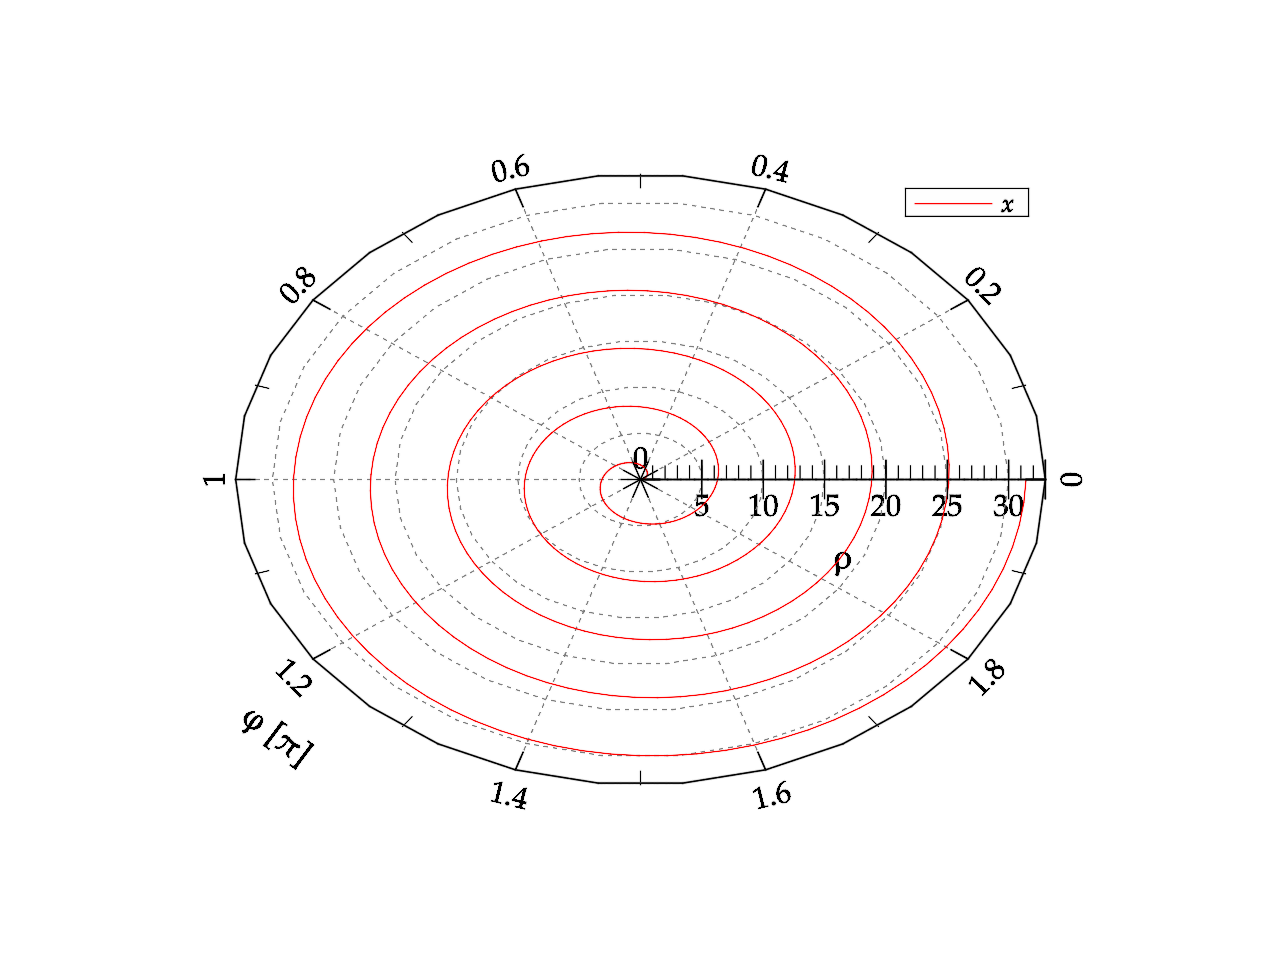
\includegraphics[width=0.45\textwidth]{_graphics/plot_7.png}}\\
					\subfloat[\lstinline{surf} with \lstinline{light}]{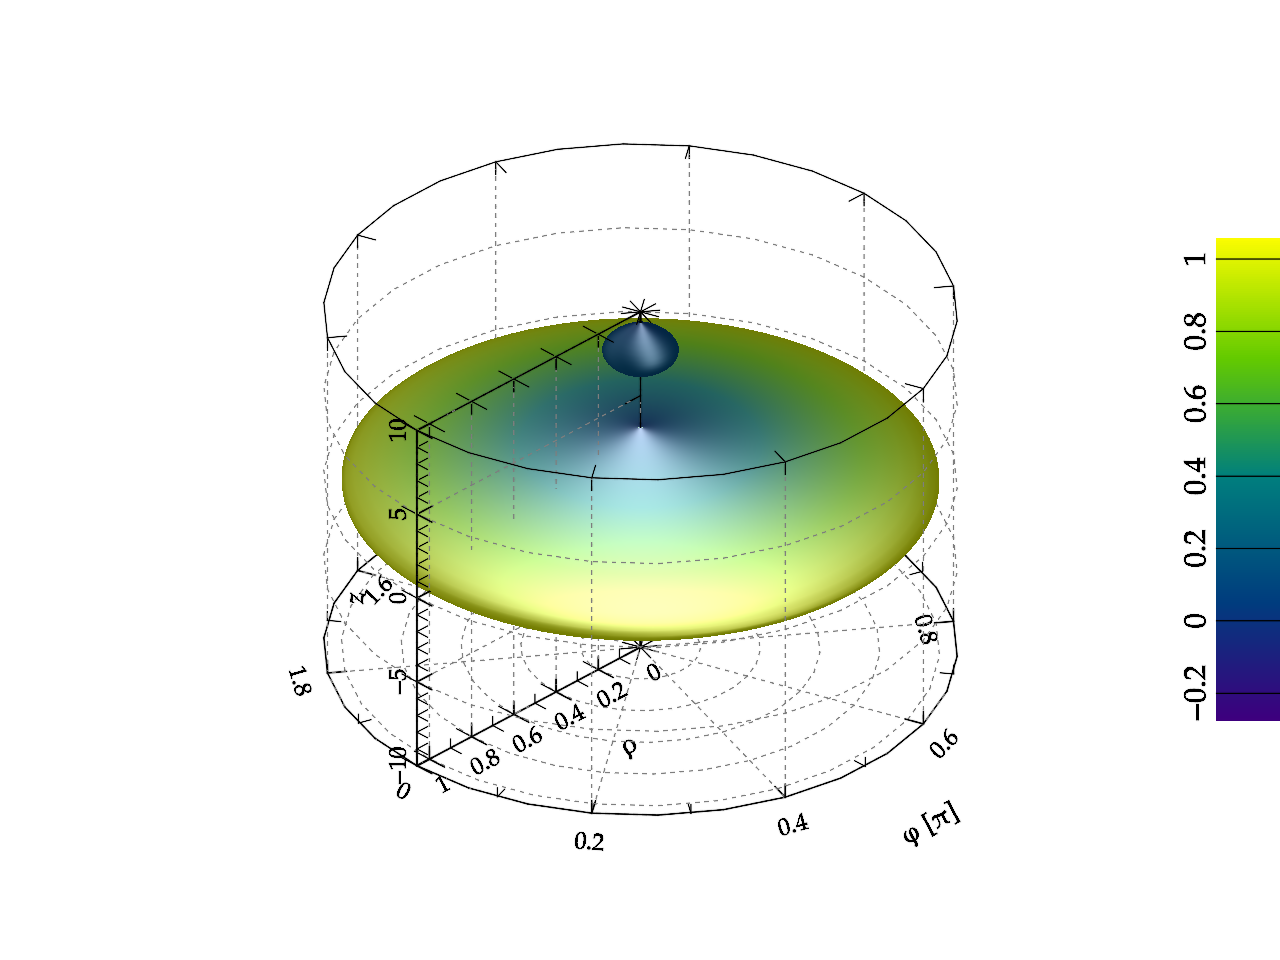
\includegraphics[width=0.45\textwidth]{_graphics/surf_0.png}}
					\subfloat[with \lstinline{coords=spherical}]{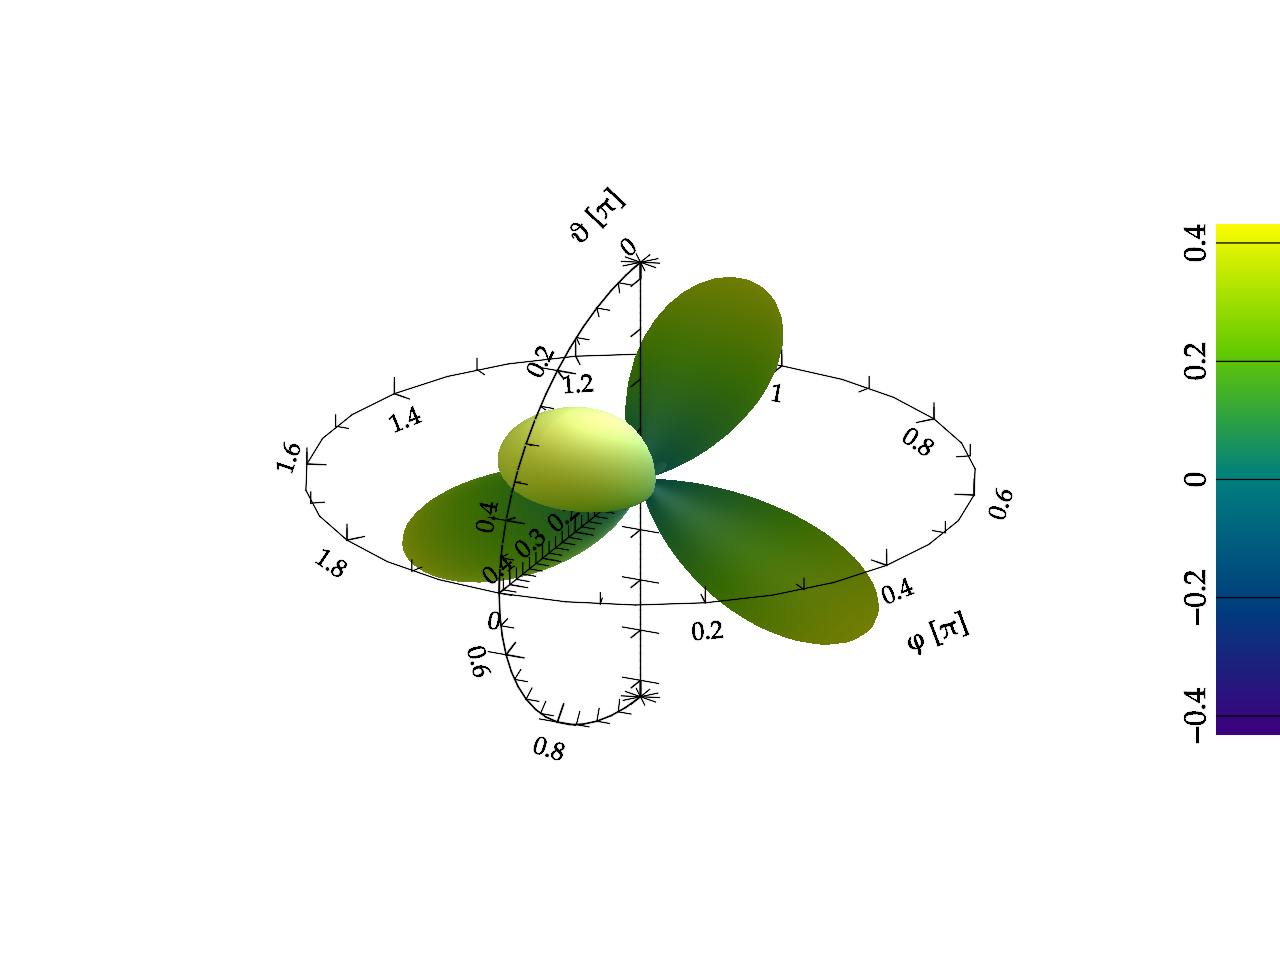
\includegraphics[width=0.45\textwidth]{_graphics/surf_1.png}}
					\caption{Results of the different coordinate systems}
					\label{fig:coords}
				\end{figure}
				
				To change the coordinate system, one uses the option \lstinline+coords=COORDINATES+. For example: to switch to polar coordinates, one passes the following line (\autoref{fig:coords}a):
				\begin{lstlisting}
plot x -set coords=polar
				\end{lstlisting}
				
				It's noticable that the variable $x$ is used as $\varphi$ and the functions value $y$ as the radial coordinate $\varrho$. The azimuthal axis is displayed in units of $\pi$, but may be changed with the option \lstinline+xscale=SCALE+, if desired. 
				
				If one changes the interval for $x$ (meaning $\varphi$), one gets the result of \autoref{fig:coords}b with the following line:
				\begin{lstlisting}
plot x -set coords=polar [0:10*_pi]
				\end{lstlisting}
				It's possible an advantage, to enlarge the number of samples with \lstinline+samples=WERT+.
				
				In combination with three-dimensional plotting functions, one switches automatically into the cylindrical system, e.g. through
				\begin{lstlisting}
surf sinc(norm(y)) -set light
				\end{lstlisting}
				one gets \autoref{fig:coords}c. The added option \lstinline+light+ activates the three-dimensional lighting, which emphasises the volume of the plot.
				
				It's getting obvious in this case that the variable $y$ has been used as $z$ and the function value $\Phi(x,y)$ has been interpreted as the radial variable $\varrho$.
				
				Last but not least, the spherical coordinate system shall be presented here. One switches with
				\begin{lstlisting}
surf Y(3,2,y,x) -set coords=spherical
				\end{lstlisting}
				to this system and creates the neat Spherical Harmonics (its real part) $Y_{3\,2}(\vartheta,\varphi)$ in \autoref{fig:coords}d. In this coordinate system $y$ is used as $\vartheta$, $x$ is again $\varphi$ and the function value $\Phi(x,y)$ is presented through the radial coordinate $r$.
				
				\paragraph{Note}
					Please note that the presented axis assignment may be changed. This can be done with the following options:
\begin{lstlisting}
polar_pz
polar_rp
polar_rz
spherical_pt
spherical_rp
spherical_rt
\end{lstlisting}
				
				\helpidx{coords}
		\chapter{Tables: the Cache}
			\NR\ manages large datasets as tables. As previously mentioned, the default table for loaded data is \lstinline+data()+. However, this table is \emph{read only}. If you need a table, which you may modify to your needs, you've to use the so-called \emph{caches}.
			\section{Concept}
				Caches are tables in \NR, whose content---similar to usual variables---may be modified freely. Their sizes are arbitrary and fit always to the needs of the user. As default, the default cache \lstinline+cache()+ already exists. You may also add additional caches.
				
				Caches are autosaving their contents. If the content of a cache is altered, these changes are saved to an external file after the autosave interval is passed. The caches and their contents are automatically recreated after a restart so that you can continue your work immediately.
			\section{Creating and Removing Caches}
				You can use the command \lstinline+new+ to create new caches (this command may also create further objects):\cmd{new}
				\begin{lstlisting}
new CACHE1(), CACHE2(), CACHE3(), ...
new amplitude(), phase(), results()
				\end{lstlisting}
				You may use the created caches just like the standard \lstinline+cache()+. If one or more caches of the list are already existing, \NR\ won't change them in any way.
				
				\helpidx{new}
				Custom created caches may also be removed, if their memory is not needed any more for further calculations:\cmd{remove}
				\begin{lstlisting}
remove CACHE1(), CACHE2(), CACHE3(), ...
remove amplitude(), phase(), results()
				\end{lstlisting}
				However, the memory, which is occupied by \NR, is only freed after a restart.
				
				\helpidx{remove}
				You may also rename caches instead of removing them:\cmd{rename}
				\begin{lstlisting}
rename -CACHE1=NEWNAME
rename -amplitude=phase
				\end{lstlisting}
				
				To remove all caches at once and free the complete memory, you may use 
				\begin{lstlisting}
clear cache()
				\end{lstlisting}
				This will also free all the occupied memory of \NR. If you only want to delete the contents of a cache, just use \cmd{delete}
				\begin{lstlisting}
delete CACHE(i1:i2,j1:j2)
				\end{lstlisting}
				
				\helpidx{cache}
			\section{Usage}
				You may use caches similar to the \lstinline+data()+ table. The central difference is the fact that the contents of caches may be altered. This means, you can also assign new values similar to variables to their elements:\cmd{cache()}
				\begin{lstlisting}
CACHE(:,1) = VALUE1, VALUE2, VALUE3, ...
CACHE(4,5:) = data(:,1)
CACHE(:,1) = CACHE(2,:)
				\end{lstlisting}
				The new values replace the already available values in \lstinline+CACHE()+.
				
				At all location, where we used \lstinline+data()+ previously, you may also use caches with the identical syntax. Internally there's no difference (except of the possibility of changing elements) between \lstinline+data()+ and the caches:
				\begin{lstlisting}
hist cache(:,1)
stats cache()
fit cache(:,4:5) -with=A*sin(B*x+C) params=[A=1, B=1, C=0]
				\end{lstlisting}
				
				Data, which is created by some commands (e.g. \lstinline+datagrid+), is sometimes written automatically to \lstinline+cache()+. Also, some of the commands are creating their target caches by themselves.
			\section{Sorting, Smoothing and Resampling}
				Sometimes one has to modify the data points further that one can reasonable process them. \NR\ offers the possibility to sort, smooth or resample (change the number of data points) the data.
				
				The data in a cache (and in principle also in \lstinline+data()+) may be sorted ascending or descending. In the following one might find distinct thresholds or points of interest in the measured data more easily.
				
				Through entering\cmd{sort}
				\begin{lstlisting}
sort -CACHE
				\end{lstlisting}
				the whole cache \lstinline+CACHE+ is sorted ascending. To sort it descending, one has to use the value \lstinline+desc+
				\begin{lstlisting}
sort -CACHE=desc
				\end{lstlisting}
				Using the option \lstinline+cols+ to columns, which shall be sorted, may be selected. In addition one may select a group of columns, which shall be sorted according an index column (if, for example, $x$ values and their function values are sorted arbitrary, the function values may be sorted according to the $x$ values without losing the connection between the  $x$ values and the function values):
				\begin{lstlisting}
sort -CACHE cols=COLUMNS[COLUMNGROUPS]
sort -cache cols=5[2:4]
				\end{lstlisting}
				
				\helpidx{cache}
				In addition to sorting the data, the data points in a cache may be freed from noise and comparable artifacts. This is achieved through smoothing the data points.
				
				The command\cmd{smooth}
				\begin{lstlisting}
smooth CACHE(i1:i2,j1:j2) -order=ORDER
				\end{lstlisting}
				smooths the cache \lstinline+CACHE+ in the selected range, where the data points are interpolated linearily over \lstinline+ORDER+ data points. \NR\ will smooth the data in two dimensions automatically, if this is reasonable according to the selected range. To switch this to column- or linewise smoothing, one may pass the options \lstinline+lines+ and \lstinline+cols+.
				
				Smoothing is in principle similar to applying a low-pass filter. If high-frequent data is of interest, smoothing will destroy this information partly or sometimes completely. As a test one might subtract the smoothed from the noisy data and plot the result. If only noise was removed, the plot should only display noise as well.
				
				\helpidx{smooth}
				To alter the number of data points (e.g. if the sample rate is not fitting or one wants to combine different data rows) \NR\ may interpolare further samples into the data or remove them as well.
				
				You'll achieve this with\cmd{resample}
				\begin{lstlisting}
resample CACHE(i1:i2,j1:j2) -samples=SAMPLES
				\end{lstlisting}
				The number of samples is altered columnwise to \lstinline+SAMPLES+. If \lstinline+SAMPLES+ is larger than the selected range, no information is lost, because the new data points are interpolated from the previous ones. If the number is smaller, of course information is lost.
				
				\helpidx{resample}
			\section{Statistics Functionalities}
				Caches (and the \lstinline+data()+ table as well) may execute global statistics operations on the data (similar to \lstinline+stats+ and statistics functions \lstinline+std()+, \lstinline+avg()+, \ldots). One has to use the caches as a command and append the desired statistics function as a parameter (there are no parentheses in the expression in this case):
				\begin{lstlisting}
CACHE -avg
CACHE -std
...
				\end{lstlisting}
				This calculates the average/standard deviation/etc. of the whole table as a single value. The additional options may be restricted further: the option \lstinline+grid+ calculates the statistics and considers the cache as a datagrid. The option \lstinline+cols+ calculates the values column- and \lstinline+lines+ linewise. The options \lstinline+lines+ and \lstinline+cols+ may be combined with \lstinline+grid+.
		\chapter{NumeRe Scripts}
			\NR\ scripts provide the possibility to outsource complex calculations and repeated analyses into a file, from where they may be easily and repeatedly executed.
			\section{Concept}
				The concept building the basis for \NR\ scripts is quite easy: all entries, which one might enter into the \NR\ console, are typed into a textfile instead, which will be read by \NR\ afterwards. \NR\ will execute the expressions and commands in the corresponding order and evaluate them.
				
				The advantage is obvious: the order of commands may easily be repeated and errors may corrected fastly without having to retype erverything.
				\paragraph{Note}
					We will talk about \NR\ procedures in a later chapter. These represent the programmability of \NR. However, most problems, which do not need too complex abstractions, may be solved using \NR\ scripts.
				
				\helpidx{script}
			\section{Syntax Highlighting}
				The syntax of \NR\ scripts is highlighted automatically, if the file was saved with the extension >>.nscr<<. It's a central part of the \NR\ editor. It provides highlighting of syntax elements, of matching parentheses and control flow blocks (e.g. \lstinline+if ... else ... endif+).
				
				Everybody is free to change the colours of the syntax highlighting to his or her need. This may be done in the options dialogue, which is available in the tools menu, at the tab >>Style<<. 
			\section{A Simple Script}
				As example, a simple script is presented here.
				
				To create a \NR\ script fast and easily, one uses the corresponding item in the file menu or click on the tool in the toolbar or enter 
				\begin{lstlisting}
new -script=first
				\end{lstlisting}
				into the \NR\ console. A \NR\ script with the name >>first.nscr<< is created in \lstinline+<scriptpath>+, which is in the first two cases opened automatically in the editor. In the latter case the line\cmd{edit}
				\begin{lstlisting}
edit first.nscr
				\end{lstlisting}
				opens the \NR\ script in the \NR\ editor so that it may be edited. (The file extension is here necessary, because \lstinline+edit+ would look for the script in the wrong directory.) Between the both text blocks in the script one enters the following lines:
				\begin{lstlisting}
## Delete the contents of the cache completely
delete cache() -ignore

## Create random numbers
random -lines=1e5 cols=2 distrib=uniform mean=0.5 width=1

## Are the number inside of the circle of unity?
cache(:,3) = (cache(:,1)^2+cache(:,2)^2) <= 1 ? true : false;

## Calculate pi
4*sum(cache(:,3))/1e5
				\end{lstlisting}
				where \lstinline+##+ starts a line comment, which is ignored by \NR (Alternatively one may use \lstinline+#*...*#+ as a block comment). The option \lstinline+ignore+ in the second line suppresses the confirmation, if one is sure that the contents of the cache shall be deleted. \cmd{random}\lstinline+random+ creates random numbers and writes them into the cache. In this case, two times 100,000 equally distributed random numbers are created in the interval $[0;1]$.
				
				The third expression is the trickiest. Here the result of a condition is written to the third column of \lstinline+cache()+. If written with words, this means something like
				\begin{quotation}
					\noindent\emph{>>If the length of the vector is smaller or equal to 1, then write >>true<<, otherwise write >>false<< to the cache.<<}
				\end{quotation}
				The so-called \emph{ternary} operator
				\begin{lstlisting}
CONDITION ? TRUE_VALUE : FALSE_VALUE
				\end{lstlisting}\cmd{()? \ldots\ : \ldots}
				is an abbreviation for the \lstinline+if...else...endif+ fork, which is explained in a later chapter. The advantage of the \emph{ternary} is that it may be executed faster but it cannot contain commands. A list of all possible logical expressions is obtained through
				\begin{lstlisting}
list -logic
				\end{lstlisting}
				At the end of this line one finds a semicolon \lstinline+;+. This suppresses the output of its result to the \NR\ console.
				
				The whole \NR\ script is a really simple \emph{Monte-Carlo} simulation. Points are placed arbitrary into a square of the length 1 and afterwards it's counted, how many of them are located in the circle of unity, which is part of this square. Assuming that the probability for each point in the square is equal, the relation of the number of all points to the number of points in the circle of unity has to be equal to $\pi/4$.
				
				If one executes the \NR\ script by either clicking on >>Execute<< or through entering the command\cmd{start}
				\begin{lstlisting}
start first
				\end{lstlisting}
				(the evaluation of \lstinline+random+ takes a moment), one gets results similar to
				\begin{lstlisting}
3.1364
3.13668
3.1454
3.13952
...
				\end{lstlisting}
				These numbers are quite near to $\pi$, although they are created through a smart usage of random numbers.
				
				If one enlarges the number of random numbers (e.g. \lstinline+1e6+ instead of \lstinline+1e5+) the approximation gets even more precise. However, the cache doesn't support an arbitrary number of elements. For even larger numbers one has to use other ways of calculating.
	\part{Advanced Usage}
		\chapter{Definition of Custom Functions}
			\NR\ already contains a large number of predefined functions (see \lstinline+list -func+). However, it's sometimes useful and practicable, if one may define his own functions, which are e.g. combining already existing ones. \NR\ may store up to 100 custom defined functions.
			\section{Definition}
				\cmd{define}A custom function is defined using
				\begin{lstlisting}
define my_function(ARGS) := EXPRESSION(ARGS)
				\end{lstlisting}
				This line creates the function \lstinline+my_function()+, which combines the complex expression of the arguments. The names and the number of arguments may be chosen arbitrary, as long as the number of arguments is not larger than 10. If the last argument of the function is called >>\lstinline+...+<<, one may pass from one to an arbitrary number of values for this argument. You have to ensure that the defined expression is able to handle an arbitrary number of values, e.g.:\cmd{"\ldots"\:}
				\begin{lstlisting}
define my_function(x,...) := x*sum(...)
				\end{lstlisting}
				
				The name of the function may be chosen freely, while ensuring that it doesn't start with a number nor is identical to a (pre-)defined function.
				
				\cmd{redefine}With
				\begin{lstlisting}
redefine my_function(ARGS) := NEW_EXPRESSION(ARGS)
				\end{lstlisting}
				the function \lstinline+my_function()+ may be redefined. The number of arguments of course doesn't have to be identical to the previous definition.
				
				Custom defined functions may be supported by comments, which illustrate, what the purpose of the function is. This comment is displayed together with the definition at
				\begin{lstlisting}
list -define
				\end{lstlisting}
				
				The comment may be added to the definition with´
				\begin{lstlisting}
define my_function(ARGS) := EXPRESSION(ARGS) -set comment="COMMENT"
				\end{lstlisting}
				or passed later with \lstinline+redefine+.
				
				\helpidx{define}
				\cmd{undefine}To remove custom defined functions, you may use the command
				\begin{lstlisting}
undefine my_function()
				\end{lstlisting}
				However, the function storage is cleared at the end of the application automatically. If one wants to prevent this behavior, one may either enter
				\begin{lstlisting}
define -save
				\end{lstlisting}
				and the follwing line after the restart
				\begin{lstlisting}
define -load
				\end{lstlisting}
				to load the functions, or one activate the automatic definition management through
				\begin{lstlisting}
set -defcontrol=true
				\end{lstlisting}
				
				\helpidx{set}
			\section{Conditioned Definition}
				In \NR\ scripts it may be an advantage, if \NR\ won't always raise an error that a function, which shall be defined in that script, is already existing. One possible solution for this case is using the command \lstinline+redefine+, another is using\cmd{ifndefined}
				\begin{lstlisting}
ifndefined my_function(ARGS) := ...
				\end{lstlisting}
				instead. The function is now only defined, if it isn't already available in the function storage.
			\section{Usage}
				A custom defined function may be used just like the predefined functions, because it is transformed in its definition internally before its execution. Therefore the calls to
				\begin{lstlisting}
my_function(1,2,3)
				\end{lstlisting}
				and 
				\begin{lstlisting}
sin(1)+cos(2)+sinc(3)
				\end{lstlisting}
				are identical for the definition
				\begin{lstlisting}
define my_function(x,y,z) := sin(x)+cos(y)+sinc(z)
				\end{lstlisting}
				You may also pass a lesser number of values as the function has arguments. \NR\ will replace the missing ones automatically with \lstinline+0+.
		\chapter{Character Strings}
			\NR\ may handle character string in addition to numerical values. First introduced to format the column titles of the tables, character strings are now a major and elaborate part or \NR's architecture.
			\section{Concept}
				Character strings (\emph{strings} for short) are successive chains of characters, which are not interpreted as variables or numerical values by \NR. To achieve this, strings have to be entered as enclosing quotation marks:
				\begin{lstlisting}
"This is a string."
				\end{lstlisting}
				The actual content of the string are all characters between the quotation marks. As a consequence, the string \lstinline+""+ is empty and has the length 0.
				
				Strings may be modified by special functions: there are functions for converting upper- to lowercase letters (or the other way around), for searching strings inside of strings, to extract a string from another string, to replace strings inside of another one, etc. The main advantage of character strings is the possibility, to format the output and to automate the processing of many files (and they are a precondition for the programming with \NR\ procedures).
				
				\helpidx{string}
			\section{Variable Type}
				The variable type for strings is the third variable type (next to numericals and tables) in \NR. Numerical variables may neiter be converted to string variables nor the other way around. However, there values may (see below).
				
				\NR\ recognizes new string variables automatically using the declaration. This declaration has to be---in contrast to numerical variables, which may be done \emph{on-the-fly}---\emph{always} be followed by a string value (at least an empty string):
				\begin{lstlisting}
numerical_variable = 3.1415926
also_numerical
string = "Hello World!"
also_string = ""
				\end{lstlisting}
				A declaration with the return value of a string function is also possible.
				
				In addition to the string variables, \NR\ knows the \cmd{string()}\lstinline+string()+ object. This is in principle a single column table, which may contain an arbitrary number of strings. The interval syntax may be used in the argument parentheses to extract a range of strings or a single value. If the argument parentheses are kept empty, the last written string is used automatically.
				
				\helpidx{string}
				Using strings one may modify the column heads of \lstinline+data()+ and the caches. This is achieved through entering\cmd{data(\#,:)\\cache(\#,:)}
				\begin{lstlisting}
data(#,1) = "Column heading 1"
cache(#,:) = "Column 1", "Column 2", "Column 3"
				\end{lstlisting}
				As you can see, you may use the interval syntax in this context, too. The hash sign \lstinline+#+ references the column headings.
				
				\helpidx{cache}
			\section{Conversion}
				The value of a string variable may be transformed to a numerical value and the other way around. The content of a string will be interpreted as a new variable, as an expression or even as a command, if applicable. Two functions exist for this purpose:
				\begin{lstlisting}
to_value()
to_cmd()
				\end{lstlisting}
				The function \lstinline+to_value()+ converts the passed string to a ma\-the\-ma\-tic\-al-nu\-me\-ri\-cal expression and evaluates it correspondingly. \lstinline+to_cmd()+ transforms the string directly to a command expression.
				
				The inverted conversion may be done in different ways:\cmd{\#VAR\\\#(EXPRESSION)}
				\begin{lstlisting}
#VAR
#(EXPRESSION)
valtostr(EXPR,C,N)
to_string()
string_cast()
				\end{lstlisting}
				The syntax \lstinline+#VAR+ or \lstinline+#(EXPRESSION)+ evaluates the following expression/variable and transforms the numerical value directly to a string. Between \lstinline+#+ and the expression one or more \lstinline+~+ may be inserted, which will add zeros in front of the value until the corresponding number of characters plus one for the \lstinline+#+ is reached. The function \lstinline+valtostr()+ is doing similar, although it's more versatile, because one may pass the filling character through the character \lstinline+C+.The function \lstinline+to_string()+ transforms everything, which isn't a string, directly to a string without evaluating it and \lstinline+string_cast()+ transforms even string variable names into strings.
		\chapter{Loops and Forks as Control Flow Statements}
			The evaluation of \NR\ scripts (and the in one of the following chapters introduced \NR\ procedures) may sometimes be simplified drastically by introducing loops and forks. (However, loops and forks are also usable directly from the \NR\ console.)
			\section{Forks}
				A fork is a location in a script, where the further evaluation of the script depends on the evaluation of a condition. Such forks are represented through the following construct:\cmd{if ()\\\ldots\\elseif ()\\\ldots\\else\\\ldots\\endif}
				\begin{lstlisting}
if (CONDITION1)
	EXECUTE, IF TRUE
elseif (CONDITION2)
	EXECUTE, IF CONDITION1 IS FALSE AND CONDITION2 IS TRUE
else
	EXECUTE, IF ALL CONDITIONS ARE FALSE
endif
				\end{lstlisting}
				
				A fork has to be composed at least out of a \lstinline+if ()+ and a closing \lstinline+endif+. In between an arbitrary number of \lstinline+elseif ()+ and at most one \lstinline+else+ as \emph{fallback case} may be used, where the \lstinline+else+ case has to be the last case before the closing \lstinline+endif+. A fork, which is only composed out of a \lstinline+if ()+ and a \lstinline+endif+, will only be executed, if the condition evaluates to true, otherwise it is ignored completely.
			
				The blocks between \lstinline+if ()+, \lstinline+endif+ and the other keywords may contain an arbitrary number of commands and expressions. In addition, these blocks may contain further loops and forks.
				
				\helpidx{if}
			\section{Conditioned Loops}
				\cmd{while ()\\\ldots\\endwhile}A conditioned loops will only be executed, as long as the condition evaluates to true. The syntax is as follows
				\begin{lstlisting}
while (CONDITION)
	EXECUTE, AS LONG AS TRUE
endwhile
				\end{lstlisting}
				In the contained block commands and/or expressions or even further loops and forks may be used.
				
				\helpidx{while}
			\section{Counting Loops}
				The execution of a counting loop depends on the value of a index variable. Using the interval syntax, a starting and an ending value have to be passed. If the ending value is \emph{smaller} than the starting value, the counting loop will count backwards automatically. After each single loop pass the index value is increased (or decreased, if the loop counts backwards) by one automatically. The index can be used in the execution block of the loop as a usual variable.
				
				The syntax of a counting loop is as follows:
				\cmd{for ()\\\ldots\\endfor}\begin{lstlisting}
for (INDEX = START:END)
	EXECUTE, AS LONG AS INDEX IS IN [START;END]
endfor
				\end{lstlisting}
				Similar to the other control flow statements, one may use commands, expressions and even further loops and forks in the execution block. After the termination of the counting loop, the index variable will be deleted automatically, if it didn't already exist before the loop.
				
				\helpidx{for}
			\section{Further Control Flow Statements}
				You may influence the execution of a loop with the both commands\cmd{continue\\break}
				\begin{lstlisting}
continue
break
				\end{lstlisting}
				\lstinline+continue+ jumps over the remaining part of the current execution block and starts a new loop pass. The command \lstinline+break+ cancels the loop completely and jumps the surrounding execution block. If the surrounding execution block is outside of any loop or fork, the whole loop or fork is terminated. A reasonable application of these commands is using them in the execution block of a fork.
				
				\helpidx{if}
		\chapter{Matrix Operations}
			\NR\ was created as a table calculation, because it's much more probable that one has to process measurement data instead of processing some matrix opertions. However, \NR\ may also do so and evaluate matrix expressions.
			\section{Execution of Matrix Operations}
				Matrix operations can only be executed in the context of the \lstinline+matop+ or \lstinline+mtrxop+ command\cmd{matop} (those are synoymes). This command starts an expression, which shall be processed using matrix operations, where the actual matrices are realized as excerpts from caches or data files or special functions. But note that as default all evaluations are still executed elementwise (even the multiplication of two matrices).
				\begin{lstlisting}
matop CACHE(i1:i2,j1:j2) * DATA(i1:i2,j1:j2) + CACHE(:,:) / ...
				\end{lstlisting}
				
				To process a matrix-matrix or matrix-vector multiplication, one has to use the \lstinline+**+\cmd{... ** ...} operator. This operator has a higher priority than all other operators, so it might be necessary to use parentheses correspondingly. In addition it is important that the dimensions of the matrices are matching each other in the context of matrix multiplication.
				\begin{lstlisting}
matop CACHE() ** (DATA() * CACHE())
				\end{lstlisting}
				
				If one doesn't provide a target cache for \lstinline+matop+, where the result may be stored, the cache \lstinline+matrix()+ is used automatically. In this case the contents of \lstinline+matrix()+ are overwritten completely.
				
				\helpidx{matop}
			\section{Special Functions}
				Special or temporary matrices or advanced matrix operations may be done with the following functions, if they are used inside of the \lstinline+matop+ command.
				\begin{itemize}
					\item \lstinline+cross(MAT)+ calculates the $n$ dimensional cross product (vector product) of the vectors, which form the $n-1$ columns of the matrix \lstinline+MAT+.
					\item \lstinline+det(MAT)+ calculates the determinant of the matrix \lstinline+MAT+, if \lstinline+MAT+ is a square matrix.
					\item \lstinline+diag(x,y,z,...)+ creates a diagonal matrix with the elements \lstinline+x,y,z,...+ as main diagonal.
					\item \lstinline+diagonalize(MAT)+ diagonalizes the square matrix \lstinline+MAT+. If the calculated diagonal elements should be complex, then a $n \times 2\,n$ matrix will be returned with the real parts on the lower and the imaginary parts on the upper first diagonal.
					\item \lstinline+eigenvals(MAT)+ calculates the eigenvalues of the square matrix \lstinline+MAT+ and returns them in the shape of a vector. If the eigenvalues are complex, then they will be returned as a matrix with two columns, where the first contains the real and the second contains the imaginary part.
					\item \lstinline+eigenvects(MAT)+ calculates the eigenvectors of the square matrix \lstinline+MAT+ and returns them in the shape of a matrix, where each column is one eigenvector. If the eigenvectors are complex, then a $n \times 2\,n$ matrix will be returned with the real parts in the odd and the imaginary parts in the even columns.
					\item \lstinline+identity(n)+ creates a $n$ dimensional identity matrix.
					\item \lstinline+invert(MAT)+ inverts the matrix \lstinline+MAT+, if an inverse matrix exists.
					\item \lstinline+matfc(x,y,z,...)+ creates a matrix out of the columns \lstinline+x,y,z,...+. If the number of elements is not sufficient for the maximal dimension, the missing ones will be replaced by 0.
					\item \lstinline+matfcf(x,y,z,...)+ creates a matrix out of the columns \lstinline+x,y,z,...+. If the number of elements is not sufficient for the maximal dimension, the missing ones will be logically generated out of the already present ones.
					\item \lstinline+matfl(x,y,z,...)+ creates a matrix out of the lines \lstinline+x,y,z,...+. If the number of elements is not sufficient for the maximal dimension, the missing ones will be replaced by 0.
					\item \lstinline+matflf(x,y,z,...)+ creates a matrix out of the lines \lstinline+x,y,z,...+. If the number of elements is not sufficient for the maximal dimension, the missing ones will be logically generated out of the already present ones.
					\item \lstinline+one(n,m)+ creates a $n \times m$ matrix, which is filled with ones. If only one argument was passed, then a square matrix will be created.
					\item \lstinline+solve(MAT)+ solves the linear system of equations, which is described by the matrix \lstinline+MAT+, with the Gaussian algorithm.
					\item \lstinline+trace(MAT)+ calculates the trace of the square matrix \lstinline+MAT+.
					\item \lstinline+transpose(MAT)+ transposes the matrix \lstinline+MAT+ (column and line indices will be exchanged).
					\item \lstinline+zero(n,m)+ creates a $n \times m$ matrix, which is filled with zeroes. If only one argument was passed, then a square matrix will be created.
				\end{itemize}
				\begin{lstlisting}
matop matfc({1,2,3},{4,5,6},{7,8,9})
/ 1  4  7 \
| 2  5  8 |
\ 3  6  9 /
matop zero(2,4)
/ 0  0  0  0 \
\ 0  0  0  0 /
				\end{lstlisting}
		\chapter{Special Commands}
			This chapter shall focus on some special commands, which weren't mentioned up to here but building a great part of the functionality of \NR.
			\section{Roots}
				\NR\ may locate roots of functions and data sets using the command \lstinline+zeroes+\cmd{zeroes}. In the case of data sets this command returns the indices of the roots (or of the location, which is neares) or, if a data set for the $x$ axis was passed, the corresponding $x$ value:
				\begin{lstlisting}
zeroes DATA()
zeroes DATA() -set x=XVALUES()
				\end{lstlisting}
				
				If the roots of a function or the intersection of two functions shall be searched, a searching interval for the $x$ axis has to be specified:
				\begin{lstlisting}
zeroes f(x) -set x=x1:x2
				\end{lstlisting}
				
				Further options, which may be passed to \lstinline+zeroes+, can be found in the corresponding documentation article.
				
				\helpidx{zeroes}
			\section{Extrema}
				The command \lstinline+extrema+\cmd{extrema} is working similar to \lstinline+zeroes+. Using this command, \NR\ will locate the extrema of functions and data sets. In the case of functions, their $x$ values are returned. In the case of data sets, their indices or the $x$ values of the locations, which are describing the extrema, are returned.
				\begin{lstlisting}
extrema f(x) -set x=x1:x2
extrema DATA()
extrema DATA() -set x=XVALUES()
				\end{lstlisting}
				\paragraph{Note} Extrema are---in contrast to roots---not easy to locate---at least, if the data has some noisy parts. However, this is true in most cases, therefore \NR\ only returns the indices or the $x$ values of the minimal or maximal value instead of interpolating them. Saddle points are also not always found. This is related to the numerical algorithm, which is sensitive to sign changes (which are not available at saddle points).
				
				\helpidx{extrema}
			\section{Integration}
				\NR\ may numerically integrate functions and data sets using the command \lstinline+integrate+\cmd{integrate}, however, only functions may be integrated two-dimensionally. If a 2D integration shall be calculated is determined by the number of passed integration intervals. If only an interval for $x$ was passed, then \NR\ will calculate a one-dimensional integration. If the command string contains a second interval for $y$ then the integration is in two dimensions.
				
				The integration intervals and further options are passed Using the parameter \lstinline+-set+. Further options are for example the precision of the integration, the numerical method, if the integration shall return the function values of the integral, etc. Further details are noted in the corresponding documentation article.
				\begin{lstlisting}
integrate x^2 -set [1:2]
				\end{lstlisting}
				
				If you want to integrate data sets, you've to pass them instead of the function: if the data set contains only one column, the integral is identical to the sum. If two columns are passed, then the first is used as $x$ and the second as the corresponding $y$ values for the calculated integral.
				\begin{lstlisting}
integrate DATA(:,1)
integrate DATA(:,1:3)
				\end{lstlisting}
				
				\helpidx{integrate}
			\section{Differentiation}
				\NR\ does also provide the ability to differentiate functions numerically to the first order using the command \lstinline+diff+\cmd{diff}. Depending on the passed parameters the differentiation is calculated at the location of $x$ or for a number of \lstinline+samples+ for a complete interval.
				\begin{lstlisting}
diff sin(x) -set x=1
diff sin(x) -set [0:1]
				\end{lstlisting}
				
				In addition, \NR\ may differentiate data sets numerically. If only one column is provided, then the distance between the samples is assumed to be 1. Otherwise, the first column is used as $x$ and the second as the corresponding $y$ values.
				\begin{lstlisting}
diff DATA(:,1)
diff DATA(:,1:2)
				\end{lstlisting}
				Only the $y$ values of the differentiation is calculated. Using the option \lstinline+xvals+ the corresponding $x$ values (which are not matching to the provided ones) are calculated and returned.
				
				\helpidx{diff}
			\section{Taylor Expansion}
				With the command \lstinline+taylor+\cmd{taylor} \NR\ may approximate functions of one variable numerically with a polynomial of the order $n\geq0$ using the taylor expansion. However, this polynomial doesn't have to share more than one point (the expansion point) with the original function (this is an issue of the taylor expansion and not a numerical or algorithmic error).
	
				The approximation is done only numerically. As a result, numerical errors are unavoidable. However, they are limited for low orders of the expansion. \NR\ will calculate numerical stable coefficients up to the order of $n = 10$ (passed through the option \lstinline+n=ORDER+, default is 6). Over this limit the numerical errors are enormous and will lead to large deviations compared to an analytic determination.
				\begin{lstlisting}
taylor cos(x)*exp(-x/2) -set x=2
				\end{lstlisting}
				
				The calculated polynomial is automatically defined as a function in the function memory. Usually, \NR\ will choose the name \lstinline+Taylor(x)+, however, if the option \lstinline+unique+ was passed to the command \lstinline+taylor+, then the used function name will be much more complex, because it will contain the expression and the order of of the polynomial expansion.
				\paragraph{Note} Already existing functions, which are stored with an identical name in the function memory, are automatically overwritten by the new definition done by this command. Therefore, the option \lstinline+unique+ creates quite reliable function names, which won't interfere with other defined functions in function memory.
				
				\helpidx{taylor}
			\section{Function Values in 1D and 2D} %eval datagrid
				Using the commands \lstinline+eval+ and \lstinline+datagrid+\cmd{eval\\datagrid} \NR\ will calculate and return function values of one- or two-dimensional functions in a predefined interval and for a predefined number of samples.
				
				The command \lstinline+eval+ returns the function values of one-dimensional functions in the predefined interval. The result may be stored directly into a cache. The number of samples is predefined using the option \lstinline+samples+ (where the default is 100) and they are linearly distributed by default. Through the option \lstinline+logscale+ this distribution is switched to a logarithmic one, which may be an advantage if one plans to display them on a logarithmic $x$ axis.
				\begin{lstlisting}
eval FUNCTION(x) -set [x0:x1] OPTIONEN
eval sin(x) -set [0:_2pi] samples=200
				\end{lstlisting}
				
				\helpidx{eval}
				\NR\ needs sometimes so-called \emph{datagrids}. This is a tabular data set, where the $x$ values are stored in the first, the $y$ values are in the second and the $z$ values are stored in the remaining columns, where the number of lines has to match to the first column and the number of columns has to match to the second column.
				
				These datagrids may be created by \lstinline+datagrid+. The values for $x$ and $y$ may be passed in different ways: either as an interval in the common form \lstinline+{x0:x1,y0:y1]+ or separate through \lstinline+x=x0:x1+ or as a column/row of a data set such as \lstinline+y=data(:,3)+.
				
				For the $z$ values there are also multiple possibilities: either as a function of $x$ and $y$ ($f(x,y) = \cos(x)\exp(-y)$), as a matrix of a data set (\lstinline+cache(3:,7:100)+) or as a single column/row of a dataset (\lstinline+data(4,2:)+). \NR\ tries in the latter case to connect the defined $(x,y,z)$ points by triangulation and to create a grid using linear interpolation.
				\begin{lstlisting}
datagrid z-VALUES -x=x-VALUES y=y-VALUES
datagrid data(:,3) -x=data(:,1) y=data(:,2)
				\end{lstlisting}
				
				The parameter \lstinline+samples=SAMPLES+ is optional und defines, how many samples \NR\ shall calculate if a component of the datagrid has to be calculated. As default (just like in 2D plots) \NR\ calculates $100\times100$ samples.
				
				If the $x$ and $y$ axis of the data points are swapped ($x =$ lines, $y=$ columns), one can pass the parameter \lstinline+transpose+ to \lstinline+datagrid+ This way the datapoint matrix is transposed before the datagrid is constructed.
	
				The created datagrid is automatically saved to a free location in the cache \lstinline+grid()+ (will be created automatically, if necessary) right og already existing data and may be plotted using this cache.
				
				\helpidx{datagrid}
			\section{Fourier Transformation}
				One of the quite common evaluation algorithms in modern science is the calculation of a Fourier transformation, which may extract frequency-dependent information out of a total noisy signal.
				
				\NR\ provides an algorithm for a fast Fourier transform, which is invoked with the command \lstinline+fft+\cmd{fft} and may calculate the amplitudes of the contained frequencies of the passed data:
				\begin{lstlisting}
fft DATA()
				\end{lstlisting}
				The passed data object has to contain at least two columns: the axis values in the first column (time or frequency) and the corresponding amplitude in the second one. If three columns are passed, then they are interpreted as axis values, amplitude and phase (in this order) or---if the additional option \lstinline+-complex+ was specified---as axis values, real and imaginary part of the amplitude.
				
				\lstinline+fft+ will store the transformed data as new columns in the passed data set (or in \lstinline+cache()+, if \lstinline+data()+ was passed). The values returned are frequency, amplitude (or \emph{magnitude}) and phase. Using the option \lstinline+-complex+ the real and imaginary parts are returned instead of amplitude and phase.
				
				An inverse transformation is achieved by passing the option \lstinline+-inverse+.
				
				\helpidx{fft}
			\section{Differential Equations}
				Few of all possible ordinary differential equations may be solved analytical or through a reasonable approximation. This is the central topic of numerics, which solves the differential equations using numerical algorithms and calculate the corresponding trajectories.
				
				\NR\ provides an integration algorithm with the command \lstinline+odesolve+\cmd{odesolve}. This algorithm may numerically integrate differential equations of the first order. Because one may transform a differential equiation of the $n$-th order into $n$ equations for the first order, this is not a problem.
				
				The differential equation may be composed out of multiple equations and may form a whole system. The equations have to follow this scheme:
				\begin{lstlisting}
dy1/dx = f1(x,y1,y2,...)
dy2/dx = f2(x,y1,y2,...)
...,				
				\end{lstlisting}
				where only the functions \lstinline+f1()+ to \lstinline+fn()+ (in this order) have to be passed. \lstinline+x+ is the integration variable and \lstinline+y1+ to \lstinline+yn+ are predefined function variables, in which \NR\ stores the results of the previous integration step. All other variables are considered as parameters.
	
				Differential equations of the $n$-th order $DGL(x,y,y',y'',\ldots,y^{(n)})$ may always be transformed into $n$ equations of the first order by introducing $n-1$ additional functions: $y' = dy_1/dx = y_2, y'' = dy_2/dx = y_3, \ldots$ Such a system follows this scheme:
				\begin{lstlisting}
dy1/dx = y2
dy2/dx = y3
...
dyn/dx = DGL(x,y1,y2,...,y(n-1))
				\end{lstlisting}
	
				The results of the integration are stored per default as a table in the cache \lstinline+ode()+. The first column contains the $x$ values and the following columns the corresponding integrated function values.
				
				To pass initial values (\NR\ uses otherwise 0 as initial value), one may use the option \lstinline+fx0=INITIALVALUES+. Additionally one may select the integration method, the tolerances the number of samples and other things. Details may be found in the integrated documentation.
				\begin{lstlisting}
odesolve DGL(x,y1,y2,...) -set [x0:x1] OPTIONS
odesolve y2,-sin(y1) -set [0:20] fx0=[0,1]
				\end{lstlisting}
				\paragraph{Note} \NR\ will provide the number of function variables corresponding to the number of equations: for one equation only \lstinline+y1+ is available, for two it's \lstinline+y1+ and \lstinline+y2+, etc. If for some reason more function variables are necessary (e.g. for a vector problem), one may pass additional 0-equations. However, the function variables are considered as constants in this case.
				
				\helpidx{odesolve}
		\chapter{NumeRe Procedures}
			In addition to be written in \NR\ scripts, command sequences may also be outsources to \NR\ procedures. \NR\ procedures provide additional functionalities to solve problems more abstract. One example is the possibility to call \NR\ procedures recursively and further process their return values.
			\section{Concept}
				\NR\ procedures are in principle similar to a mixture of a custom defined function and a \NR\ script. In addition, \NR\ procedures may call themselves recursively (\lstinline+define+ would raise an error if one would try that) and evaluate more complex commands and expressions (Procedures are not restricted to expressions, which have to fit into one single line).
				
				Using \NR\ procedures it's possible to write own subprograms in \NR\ or add further functionalities as new commands (this is known as \emph{plugin}).
				
				The ideal value of a \NR\ procedure in \NR\ corresponds to the function of a usual programming language.
								
				\helpidx{procedure}
			\section{Structure}
				The structure of \NR\ procedures has three main sections: the procedure head, the procedure body and the procdure tail. The head contains the name, the argument list and additional >>flags<<, the body contains the complete commands and expressions:\cmd{procedure\\\ldots\\endprocedure}
				\begin{lstlisting}
procedure $PROCEDURE_NAME(ARGLIST) :: FLAGS  ## Procedure head
	PROCEDURE BODY                           ## Commands and expressions
endprocedure                                 ## Procedure tail
				\end{lstlisting}
				To call a \NR\ procedure, one enters \lstinline+$PROCEDURE_NAME(VARS+ in \NR\ scripts, other \NR\ procedures or the \NR\ console. The \lstinline+VARS+ should correspond to the number of arguments in \lstinline+ARGLIST+. If \lstinline+ARGLIST+ contains default values for arguments, then the values for these arguments may be omitted on \lstinline+VARS+. The default values for the corresponding arguiments are used in this case.
				
				The mentioned >>flags<< take influence on the \NR\ procedure as a whole and suppress or allow a distinct behaviour of \NR\ in this procedure. However, a correct usage of flags requires the knowledge of the following sections and chapters:\cmd{explicit\\private\\inline}
				\begin{lstlisting}
explicit
private
inline
				\end{lstlisting}
				The flag \lstinline+explicit+ suppresses the execution of plugins in this procedure, procedures with the flag \lstinline+private+ may only be called from the same namespace and procedures with the flag \lstinline+inline+ allow faster execution of loops, if only procedures of this type are used in the loops. However, \lstinline+inline+ procedures are quite restricted in their usage.
				
				Flags may be used in an arbitrary combination/order, because they do not interfere with each other.
				
				Each \NR\ procedure has to be written to its own *.nprc file, which carries the name of the procedure. Although this sounds difficult and may be a additional error source, it might be done completely by \NR\. Through the corresponding menu item in the file menu, through clicking on the button of the toolbar or through
				\begin{lstlisting}
new -proc=$PROCEDURE_NAME
				\end{lstlisting}
				a \NR\ procedure with the name \lstinline+$PROCEDURE_NAME+ is created at the default procedure storing location \lstinline+<procpath>/PROCEDURE_NAME.nprc+. By entering 
				\begin{lstlisting}
edit $PROCEDURE_NAME
				\end{lstlisting}
				the procedure \lstinline+$PROCEDURE_NAME+ may be edited in the \NR\ editor.
				
				The procedure body of a \NR\ procedure may be written just like a \NR\ script. The few differences are explained in the following sections.
			\section{Local and Global Variables}
				\NR\ procedures distinguish between local and global variables. Global variables are variables, which may be used from every procedure, every script and the \NR\ console. Local variables, in contrast, may \emph{only} be used in \emph{this} procedure and \emph{only} in \emph{this} recursion of this procedure.
				
				Local variable are declared with\cmd{var\\str\\tab}
				\begin{lstlisting}
var VARIABLES
str STRINGVARIABLES
tab CACHES
				\end{lstlisting}
				These commands may only be used once per procedure and declare a set of local numerical variables, string variables and local caches. These variables will be deleted automatically at the end of the procedure. (Local variables may be have an identical name to a global one. In the body of a \NR\ procedure the local variables have the higher priority. This behaviour is called \emph{shadowing}.)
			\section{Return Values}
				\NR\ procedures return as default the value \lstinline+true+, if the evaluation reaches the final line of a procedure: \lstinline+endprocedure+. Additionally, \NR\ procedures may also return other values if\cmd{return}
				\begin{lstlisting}
return VALUE
				\end{lstlisting}
				occurs at the corresponding line in the procedure. \NR\ will leave the procedure as soon as \NR\ reaches this command (It may be used multiple times in a procedure). \lstinline+VALUE+ may be either a numerical value or a string. Additionally one may use \lstinline+true+ and \lstinline+false+ explicitly as \lstinline+VALUE+.
				
				\lstinline+VALUE+ doesn't have to be one single value. You may also return multiple numerical values or multiple strings together. Even a combination of both variable types is possible, although another error source, because the calling procedure must be able to handle the returned set an values.
				
				If procedures with multiple return values are used for \lstinline+while+ loops or \lstinline+if+ conditions, then only the first returned value is used for the logical operations.
				
				The special value \lstinline+void+ is used to notify \NR\ that this procedure explicitly \emph{doesn't} have a return value.
			\section{Namespaces}
				\NR\ can handle namespaces similar to C++, which allow to have multiple procedures with the same name but different behaviour in different namespaces. Procedures of other namespaces than the \lstinline+main+ namespaces are called through 
				\begin{lstlisting}
$NAMESPACE~PROCEDURNAME(VARS)
				\end{lstlisting}
				The corresponding procedure \lstinline+$PROCEDURENAME+ is stored in the file 
				\begin{lstlisting}
<procpath>/NAMESPACE/PROCEDURENAME.nscr
				\end{lstlisting}
				The command \lstinline+new+ may create procedures in namespaces automatically, if that is mentioned explicitly:
				\begin{lstlisting}
new -proc=$NAMESPACE~PROCEDURENAME
edit $NAMESPACE~PROCEDURENAME
				\end{lstlisting}
				If one uses the functionalities of the graphical user interface, this is also true.
				
				If in one procedure \NR\ procedures out of a specific namespace are called more often, the one can predefine this namespace as a temporary default namespace by adding\cmd{namespace}
				\begin{lstlisting}
namespace NAMESPACE
				\end{lstlisting}
				to the procedure's body. (Procedures out of other namespaces may be still be called, by naming their namespace explicitly.)
			\section{Exception Handling}
				\NR\ procedures provide a somehow rudimentary way of handling exceptions. If an exception occurs, which may not be handled in any reasonable way (e.g. a wrong input), then the evaluation of the procedure can be aborted immediately through the command\cmd{throw}
				\begin{lstlisting}
throw
				\end{lstlisting}
				This command is passed through the whole stack until it reaches the default \NR\ console, where it produces a corresponding error message.
				
				It's somehow more informative, if one passes an explicit error message. This is done as a string
				\begin{lstlisting}
throw "This is the error message."
				\end{lstlisting}
				which is finally displayed in the \NR\ console.
			\section{Debugging}
				A \NR\ procedure will only in very few cases run without problems and be free of errors. Typos and logical errors are much too probable to avoid such kind of mistakes. During the execution of such a erroneous \NR\ procedure \NR\ will, if it's a syntax error, abort the evaluation at the position of the error. However, it won't always abort if there's an error in the calculations.
				\begin{figure}[htb]
					\centering
					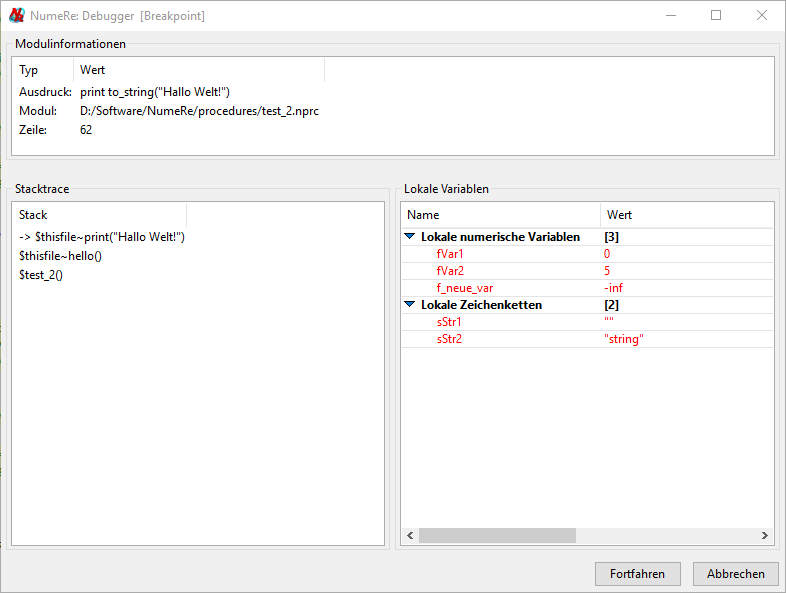
\includegraphics[width=\textwidth]{_graphics/debugger.png}%
					\caption{The \NR\ debugger at a breakpoint. Changes to the previously evaluated breakpoint are highlighted in red}%
					\label{fig:debugger}%
				\end{figure}
				
				To locate and solve such errors, \NR\ provides the so-called \NR\ debugger (\autoref{fig:debugger}). This functionality may be activated with the corresponding item in the Tools menu or through clicking on the button of the toolbar. It lists at syntax errors automatically the erroneous expression, the approximated line number, the erroneous module (the file), a stack trace and all local variables including their values of the current procedure. Using the stack trace one may reconstruct, in which procedure the error occured and which arguments were passed to this procedure.
				
				In addition to the automatic listing at syntax errors the \NR\ debugger may provide similar information at a \emph{breakpoint}. A temporary breakpoint may be set using the function of the toolbar or through clicking on the sidebar at the corresponding line. Please note that you \emph{cannot} place temporary breakpoints in empty or comment-only lines.
				
				Permanent breakpoints are set with \lstinline+|>+ at the beginning of a line, but they are seldom necessary. \NR\ stops, before the \emph{current line} is evaluated and lists stack trace and variable values. Through clicking on >>Continue<< the evaluation is continued, through clicking on >>Cancel<< the whole evaluation is aborted. (Breakpoints are of course ignored, if the debugger is not active.)
				
				\helpidx{debugger}
		\chapter{Animated Graphs}
			In some cases it's suitable that one may enhance the derivation in time of a quantity using an animated graph. \NR\ has a built-in possibility to create such an animation. However, an animation may also be created using a loop, saving every frame independent and combine all frames to an animation afterwards.
			
			To create an animation by \NR\ one has to use at least once the variable \lstinline+t+ in the expression, which shall be plotted. This variable is the time parameter, which will be varied by the animation. Additionally, one has to pass the option \lstinline+animate+ to the plotting command:\cmd{animate}
			\begin{lstlisting}
PLOTCMD EXPRESSION(t,VARS) -set animate OPTIONS
			\end{lstlisting}
			This will create an animation, which is composed out of multiple frames. In the \NR\ Graph\-Viewer one can play this animation or examine each frame independently.
			
			\helpidx{plotoptions}
			\paragraph{Note}
				\NR\ cannot create animations from datasets. The reason is that the time parameter is a floating number, whereas indices for tables are integer. To create an animation from a dataset, one has to create the frames independent using a loop.\bigskip\\
			\NR\ creates per default 50 frames per animation with a duration of $1/25$~s each and uses the interval $[0;1]$ for the time parameter \lstinline+t+. This may be altered of course, however, it's possible that too many frames will result in memory problems, because every single frame is stored in memory first:
			\begin{lstlisting}
PLOTCMD EXPRESSION(t,VARS) -set t=0:2 animate=100 OPTIONS
			\end{lstlisting}
			Now an animation with 100 frames is created and the time parameter uses the interval $[0;2]$.
			\paragraph{Note}
				Some plot types may need too many memory so that an animation is not possible. It may help to reduce the number of \lstinline+samples+ for this image.
		\chapter{Composed Graphs}
			It's possible that a desired plotting layout is only possible, if one could combine two plotting types. Using the command block\cmd{compose\\\ldots\\endcompose}
			\begin{lstlisting}
compose
	PLOTTYPE1
	PLOTTYPE2
	...
endcompose
			\end{lstlisting}
			it's possible in \NR. The \lstinline+compose+ mode may only contain plotting commands. This means that all calculations for the desired plot types have to be finished in advance.
			
			Some plot options are valid for the whole composed plot (e.g. the plot interval, the axis labels, the grid, etc.), others may be switched on or off for each plot independent (e.g. transparency, lighting, additional contour lines, errorbars, etc.). The plotting colours and the line styles may also be selected for each plot, however, one has to keep in mind that \NR\ has an internal counter, which will be incremented for each line in all plots of the composed plot. The styling information has to be adapted to deal with this behaviour.
			
			Using the \lstinline+compose+ mode one may display plots of different quantities together, e.g. a vector field together with its potential. It's not necessary to use a distinct order, \NR\ will order the plots by itself so that they are in a reasonable order:
			\begin{lstlisting}
compose
	dens 1/norm(x,y)
	vect x/norm(x,y)^3,y/norm(x,y)^3
endcompose
			\end{lstlisting}
			
			\helpidx{compose}
			The \lstinline+compose+ mode also enables to work around the restriction of a single function per 3D plot type (except of \lstinline+plot3d+), if the functions are passed in a \lstinline+compose+ environment successive 3D plots.
		\chapter{Plugins}
			Although \NR\ is constantly extended, some functionalities might not be implemented or not correspond to the desires of the \NR\ user. This is the regime of the \NR\ plugins, which may overwrite existing functionalities or add new ones.
			\section{Functionality}
				Plugins are completely integrated into the command architecture so that one might not recognize from the outside that the routines currently executed are part of a plugin. They are called through own or already existing commands (replacing their functionalities) and use the usual \NR\ syntax.
				
				Additionally, one might add a documentation article to the documentation index. So the description of the plugin is included and may be called in the usual way.
			\section{Installation}
				Plugins are published as installation routines in \NR\ scripts, which contain\cmd{<install>\\\ldots\\<endinstall>}
				\begin{lstlisting}
<install>
	DECLARATIONS AND PROCEDURES
<endinstall>
				\end{lstlisting}
				To install such a plugin one has to enter\cmd{install}
				\begin{lstlisting}
install SCRIPTNAME
				\end{lstlisting}
				into the \NR\ console (if the script is not located in \lstinline+<scriptpath>+, one has to add the path, too). \NR\ will execute the installation routine, create the corresponding procedures and generate the needed connections. It's \emph{not} possible, to install a plugin iwth the functionalities of the graphical user interface.
				
				\helpidx{install}
				After the script was finished, the plugin is installed. Now it should be listed at
				\begin{lstlisting}
list -plugins
				\end{lstlisting}
				and may be executed with the displayed command. The shown description should contain a brief information of the functionalities of the plugin.
				
				To uninstall a plugin afterwards, one enters\cmd{uninstall}
				\begin{lstlisting}
uninstall PLUGINNAME
				\end{lstlisting}
				into the \NR\ console. The \lstinline+PLUGINNAME+ is displayed at
				\begin{lstlisting}
list -plugins
				\end{lstlisting}
				in brackets next to the description. In some cases it might be necessary to enclose \lstinline+PLUGINNAME+ in quotation marks.
				\paragraph{Note}
					It's not necessary to uninstall a plugin first before a newer version of itself might be installed. The installation may be executed directly over the already existing one. \NR\ will change the corresponding connections by itself.
			\section{Custom Plugins}
				The development of custom plugins may sound complicated first, but actually it's not so difficult. \NR\ aides by creating a template for the plugin installation routine. This template is created by using the functionalities of the graphical user interface or through entering
				\begin{lstlisting}
new -plugin=PLUGINNAME
				\end{lstlisting}
				This creates a plugin with the name PLUGINNAME as a \NR\ script at
				\begin{lstlisting}
<scriptpath>/plgn_PLUGINNAME.nscr
				\end{lstlisting}
				with the main procedure
				\begin{lstlisting}
$plugins~PLUGINNAME~main(<CMDSTRING>)
				\end{lstlisting}
				This plugin template contains already all necessary installation elements (including the documentation article) with the corresponding placeholders.
				
				Plugins are composed out of one or more procedures, which represent the plugin's functionality. Together with the declaration of a plugin, a main procedure has to be named, which is called by \NR\ as soon as the plugin's command is entered. \NR\ then passes the command string in one or more of the following shapes to this procedure. The shapes (or >>tags<<) have to be named during the declaration of the plugin:\cmd{<CMDSTRING>\\<EXPRESSION>\\<PARAMSTRING>}
				\begin{lstlisting}
<CMDSTRING>
<EXPRESSION>
<PARAMSTRING>
				\end{lstlisting}
				\begin{itemize}
					\item \lstinline+<CMDSTRING>+ passes the whole command line (including the plugin's command)
					\item \lstinline+<EXPRESSION>+ passes the expression, which may be found between the command and optional parameters
					\item \lstinline+<PARAMSTRING>+ passes the parameter set, which begins either at \lstinline+-set+ (if an \lstinline+<EXPRESSION>+ is available) or at the first \lstinline+-+ after the command
				\end{itemize}
				
				The procedures, which represent the plugin's functionality have to be copied to that script. Afterwards one has to update the installation information block:\cmd{<info>\\\ldots\\<endinfo>}
				\begin{lstlisting}
<install>
	<info>
		-author="AUTHORNAME"
		-version="VERSION"
		-type=TYPE_PLUGIN
		-flags=ENABLE_DEFAULTS
		-name="PLUGINNAME"
		-pluginmain=$PLUGINMAINPROCEDURE(<CMDSTRING>)
		-plugincommand="PLUGINCOMMAND"
		-plugindesc="DESCRIPTION"
	<endinfo>
	PROCEDURES
<endinstall>
				\end{lstlisting}
				The plugin may now installed with the command \lstinline+install+ (The values for \lstinline+type+ and \lstinline+flags+ are actually uppercase letters).
				
				If the \lstinline+PLUGINCOMMAND+ is now entered into the \NR\ console, then \NR\ calls the procedure \lstinline+$PLUGINMAINPROCEDURE()+ and passes it the tag \lstinline+<CMDSTRING>+. One may also pass other or further sub expressions of the command line, if they are named as arguments of the main procedure.
				
				If the plugin shall return a value, which one may process further, then the \lstinline+type+ has to be changed to
				\begin{lstlisting}
-type=TYPE_PLUGIN_WITH_RETURN_VALUE
				\end{lstlisting}
				
				The \lstinline+version+ flag may be passed as
				\begin{lstlisting}
-version=<AUTO>
				\end{lstlisting}
				For each installation of the plugin the version number is incremented automatically. This is for example of great use during the development, if one wants to fix the version number to the number of changes.
				
				Normally, the installed procedures are logged in the console, so that the user may see, what's happening. One may also suppress this output by setting
				\begin{lstlisting}
-flags=DISABLE_SCREEN_OUTPUT
				\end{lstlisting}
				instead \lstinline+ENABLE_DEFAULTS+. Further flags are
				\begin{lstlisting}
ENABLE_FULL_LOGGING
ENABLE_FORCE_OVERRIDE
				\end{lstlisting}
				They are either logging the complete installation linewise to \lstinline+<>/install.log+ or they enable the overwriting of an already available plugin with the same command but a different author, which is prevented by default.
				
				\helpidx{plugins}
				Before \lstinline+<endinstall>+ one has the possibilty to add the information to a documentation article for the \NR\ documentation using a XML-like syntax:\cmd{<helpindex>\\\ldots\\</helpindex>\\<helpfile>\\\ldots\\</helpfile>}
				\begin{lstlisting}
<install>
	...
	PROCEDURES
	<helpindex>
		INDEXINFORMATION
	</helpindex>
	<helpfile>
		DOCUMENTATIONARTICLE
	</helpfile>
<endinstall>
				\end{lstlisting}
				The \lstinline+INDEXINFORMATION+ contain the keywords, for which \NR\ shall display the corresponding article, as well as information for the index itself, if one enters \lstinline+help idx+.
				
				The section \lstinline+DOCUMENTATIONARTICLE+ contains the actual documentation and description of the installed plugin.
				
				\helpidx{documentation}
				%

\end{document}